\documentclass[12pt]{article}

\usepackage[margin=3cm]{geometry}
\usepackage{graphicx}
\usepackage{booktabs}
\usepackage{microtype}
\usepackage{parskip}
\usepackage{float}
\usepackage[section]{placeins}
\usepackage{caption}
\usepackage{subcaption}
\usepackage{hyperref}
\usepackage{libertine}
\usepackage[libertine]{newtxmath}
\usepackage{xcolor}

\hypersetup{colorlinks=true, linkcolor=black, urlcolor=black, citecolor=black}
\setcounter{tocdepth}{2}

\setcounter{topnumber}{4}
\setcounter{bottomnumber}{2}
\setcounter{totalnumber}{6}
\renewcommand{\topfraction}{0.90}
\renewcommand{\bottomfraction}{0.50}
\renewcommand{\textfraction}{0.07}
\renewcommand{\floatpagefraction}{0.70}
\setlength{\floatsep}{6pt plus 2pt minus 2pt}
\setlength{\textfloatsep}{10pt plus 2pt minus 4pt}
\makeatletter
\setlength{\@fptop}{0pt}
\setlength{\@fpsep}{8pt}
\setlength{\@fpbot}{0pt plus 1fil}
\makeatother

\newcommand{\todo}[1]{\textcolor{red}{\textbf{[TODO: #1]}}}

\title{Cache Liveness Prediction:\\[0.4em]
       \large Characterisation, Predictor Analysis, and Replacement Policy}
\author{Oskar Tegby, Alberto Ros}
\date{\today}

\begin{document}

\maketitle

\begin{abstract}
We characterise LLC and STLB block liveness across seven benchmark suites
--- SPEC CPU2017, GAP, Ligra, Google, Qualcomm, GMS, and AI/ML ---
mirroring the workload selection of Mazumdar~2021 while extending it to
server and AI/ML traces not evaluated in the original work.
We use the resulting signal to guide two complementary mechanisms: a
page-level bypass predictor (dpPred$+$cbPred) and a liveness-guided
replacement policy (\texttt{srrip\_live}).
The LLC--STLB DoA correlation is the central explanatory variable.
It is high for SPEC (${\sim}33\%$), near zero for server workloads and
GAP (${\sim}1$--$4\%$), but unexpectedly high for Ligra and AI/ML
(approaching $100\%$) --- the streaming, uniform access patterns of
those workloads isolate dead pages from live ones at the page level.
\texttt{srrip\_live} operates at block granularity and benefits all
workload classes; the bypass predictor's effectiveness tracks the
correlation closely.
\end{abstract}

\tableofcontents

% ─────────────────────────────────────────────────────────────────────────────
\section{Definitions}
\label{sec:defs}
% ─────────────────────────────────────────────────────────────────────────────

A cache block (or STLB page) is assigned a liveness class at eviction time
based on the fraction of its residence that it was actually accessed:
\begin{equation}
  \begin{cases}
    \text{DoA (dead-on-arrival):} & \text{never accessed after insertion,} \\
    \text{mostly-dead:}           & \text{dead time} > \text{live time,}   \\
    \text{mostly-alive:}          & \text{dead time} \leq \text{live time.}
  \end{cases}
\end{equation}
The \emph{LLC--STLB DoA correlation} for a workload is defined as the
fraction of DoA LLC evictions whose physical page is also classified DoA
at the STLB:
\begin{equation}
  \text{correlation} =
    \frac{\text{DoA LLC evictions on a DoA STLB page}}
         {\text{all DoA LLC evictions}}.
\end{equation}
A high correlation means that page-level liveness (as seen by the STLB)
reliably predicts block-level liveness; near-zero correlation means the
two levels are decoupled.

Unless noted, all experiments use plain LRU as the baseline replacement
policy, no prefetcher, and the configuration from Mazumdar~2021 Table~I:
L1D~32\,KB, L2C~256\,KB (11\,cy), LLC~2\,MB (40\,cy), STLB~128~entries.
Warmup is 50\,M instructions; simulation is 100\,M instructions.

% ─────────────────────────────────────────────────────────────────────────────
\section{Liveness Characterisation}
\label{sec:liveness}
% ─────────────────────────────────────────────────────────────────────────────

\subsection{How much dead traffic is there?}

Table~\ref{tab:selected_workloads} lists the workloads selected for the
per-suite overview figures.  From each suite we keep the four workloads
with the highest combined LLC + STLB dead fraction (DoA + mostly-dead),
matching the presentation style of Mazumdar~et~al., but extended to all
seven suites.  Geomean bars are computed over all workloads in the suite,
not just the four displayed.

\begin{table}[tbp]
\caption{Selected workloads per suite (top-4 by combined LLC+STLB dead fraction).  Dead\% = DoA + mostly-dead evictions at LLC or STLB eviction;
           dashes indicate fewer than one eviction recorded.}
\label{tab:selected_workloads}
\centering\small
\begin{tabular}{llrr}
\toprule
Suite & Workload & LLC dead\% & STLB dead\% \\
\midrule
  SPEC (DPC3) & \texttt{bwaves} & 100 & 100 \\
  SPEC (DPC3) & \texttt{lbm} & 100 & 100 \\
  SPEC (DPC3) & \texttt{imagick} & 100 & --- \\
  SPEC (DPC3) & \texttt{fotonik3d} & 100 & 100 \\
\addlinespace
  GAP & \texttt{bfs-14} & 100 & 100 \\
  GAP & \texttt{bfs-10} & 99 & 99 \\
  GAP & \texttt{sssp-10} & 86 & 63 \\
  GAP & \texttt{sssp-14} & 86 & 65 \\
\addlinespace
  Ligra & \texttt{CF} & 100 & 100 \\
  Ligra & \texttt{PageRankDelta} & 100 & 100 \\
  Ligra & \texttt{BFSCC} & 100 & 100 \\
  Ligra & \texttt{BellmanFord} & 100 & 100 \\
\addlinespace
  Qualcomm (QMM) & \texttt{srv\_s7} & 92 & 81 \\
  Qualcomm (QMM) & \texttt{srv\_743} & 92 & 81 \\
  Qualcomm (QMM) & \texttt{srv\_526} & 91 & 79 \\
  Qualcomm (QMM) & \texttt{srv\_s10} & 90 & 82 \\
\addlinespace
  Google & \texttt{arizona.0} & 98 & 87 \\
  Google & \texttt{tahoe.2} & 98 & 95 \\
  Google & \texttt{charlie.1} & 98 & 89 \\
  Google & \texttt{charlie.2} & 97 & 90 \\
\addlinespace
  GMS & \texttt{tri\_cnt.137} & 100 & 99 \\
  GMS & \texttt{tri\_cnt.117} & 100 & 99 \\
  GMS & \texttt{tri\_cnt.360} & 100 & 98 \\
  GMS & \texttt{kclique\_star.1291} & 100 & 98 \\
\addlinespace
  AI/ML & \texttt{bark.1} & 100 & 100 \\
  AI/ML & \texttt{clip.1} & 100 & 100 \\
  AI/ML & \texttt{whisper.1} & 100 & 100 \\
  AI/ML & \texttt{whisper.3} & 100 & 100 \\
\addlinespace
\bottomrule
\end{tabular}
\end{table}


\begin{figure}[htbp]
  \centering
  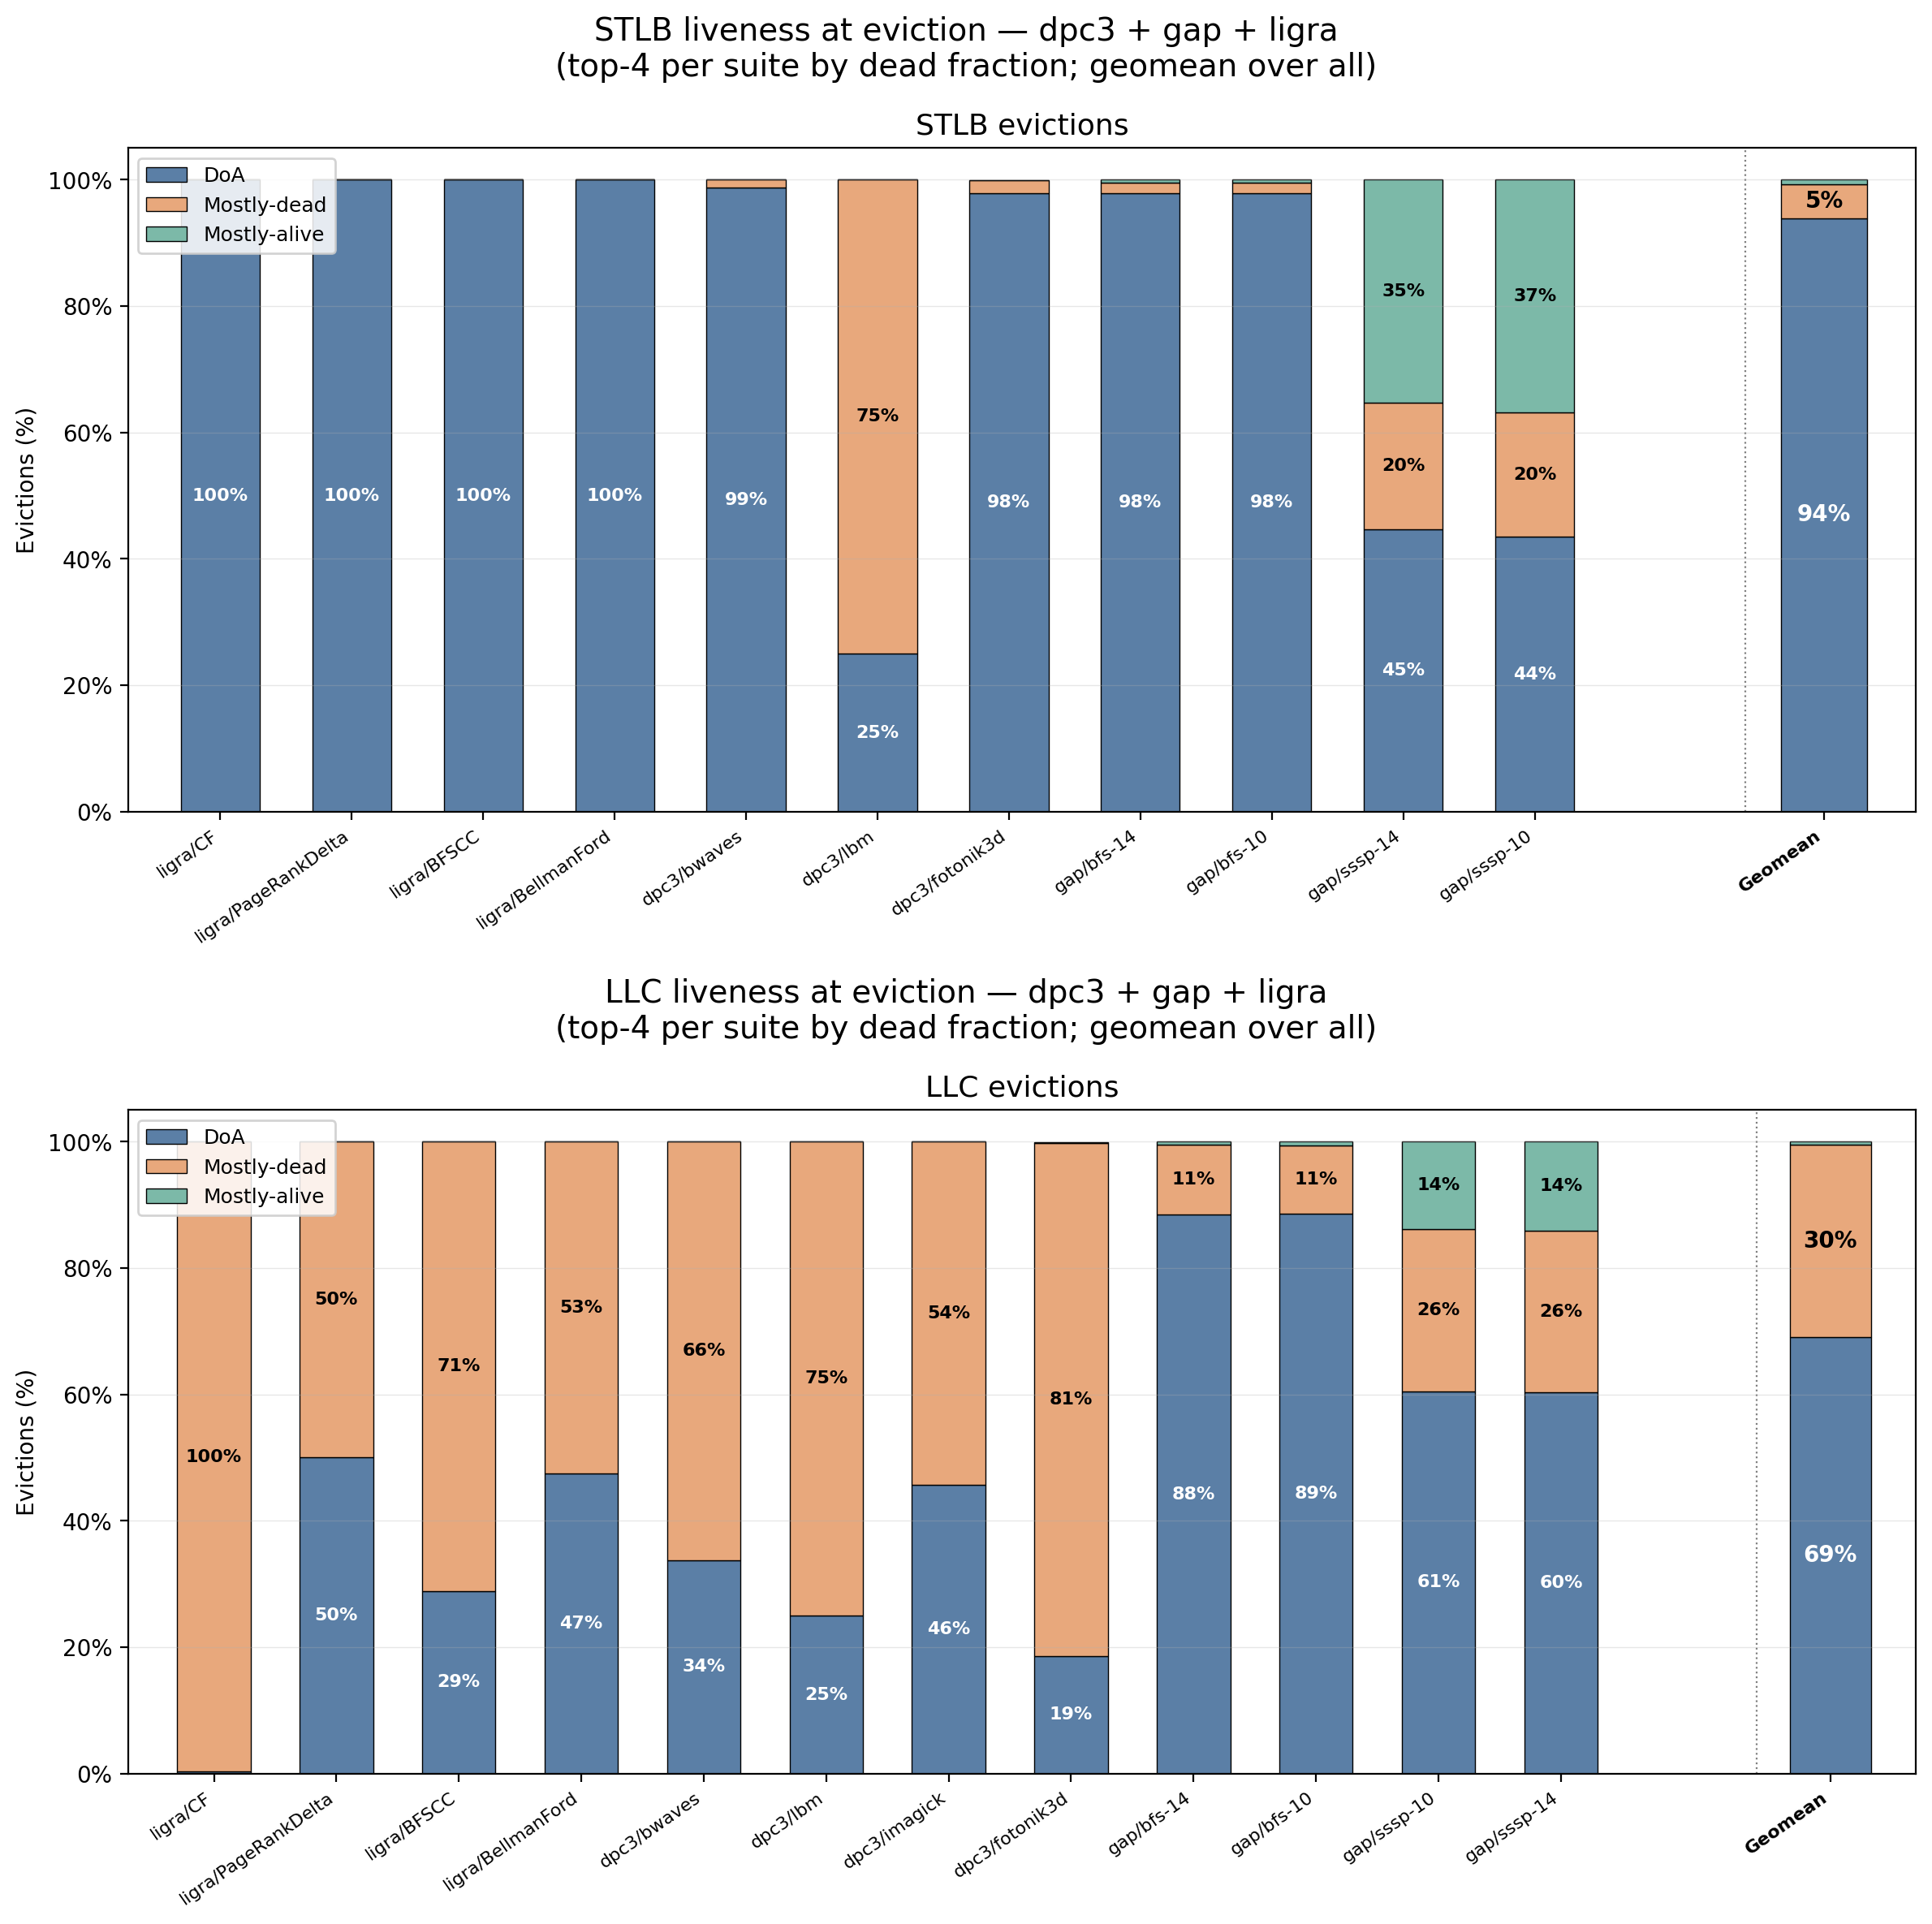
\includegraphics[width=\linewidth]{../../plots/liveness/maz_liveness_bar_all.png}
  \caption{Per-workload liveness breakdown (STLB top, LLC bottom) for the
           Mazumdar-comparable domain: SPEC (DPC3), GAP, and Ligra.
           Each bar shows one workload (top-4 per suite by dead fraction);
           rightmost bar per suite is the geomean over all suite workloads.}
  \label{fig:liveness_bar_mazumdar}
\end{figure}

\begin{figure}[htbp]
  \centering
  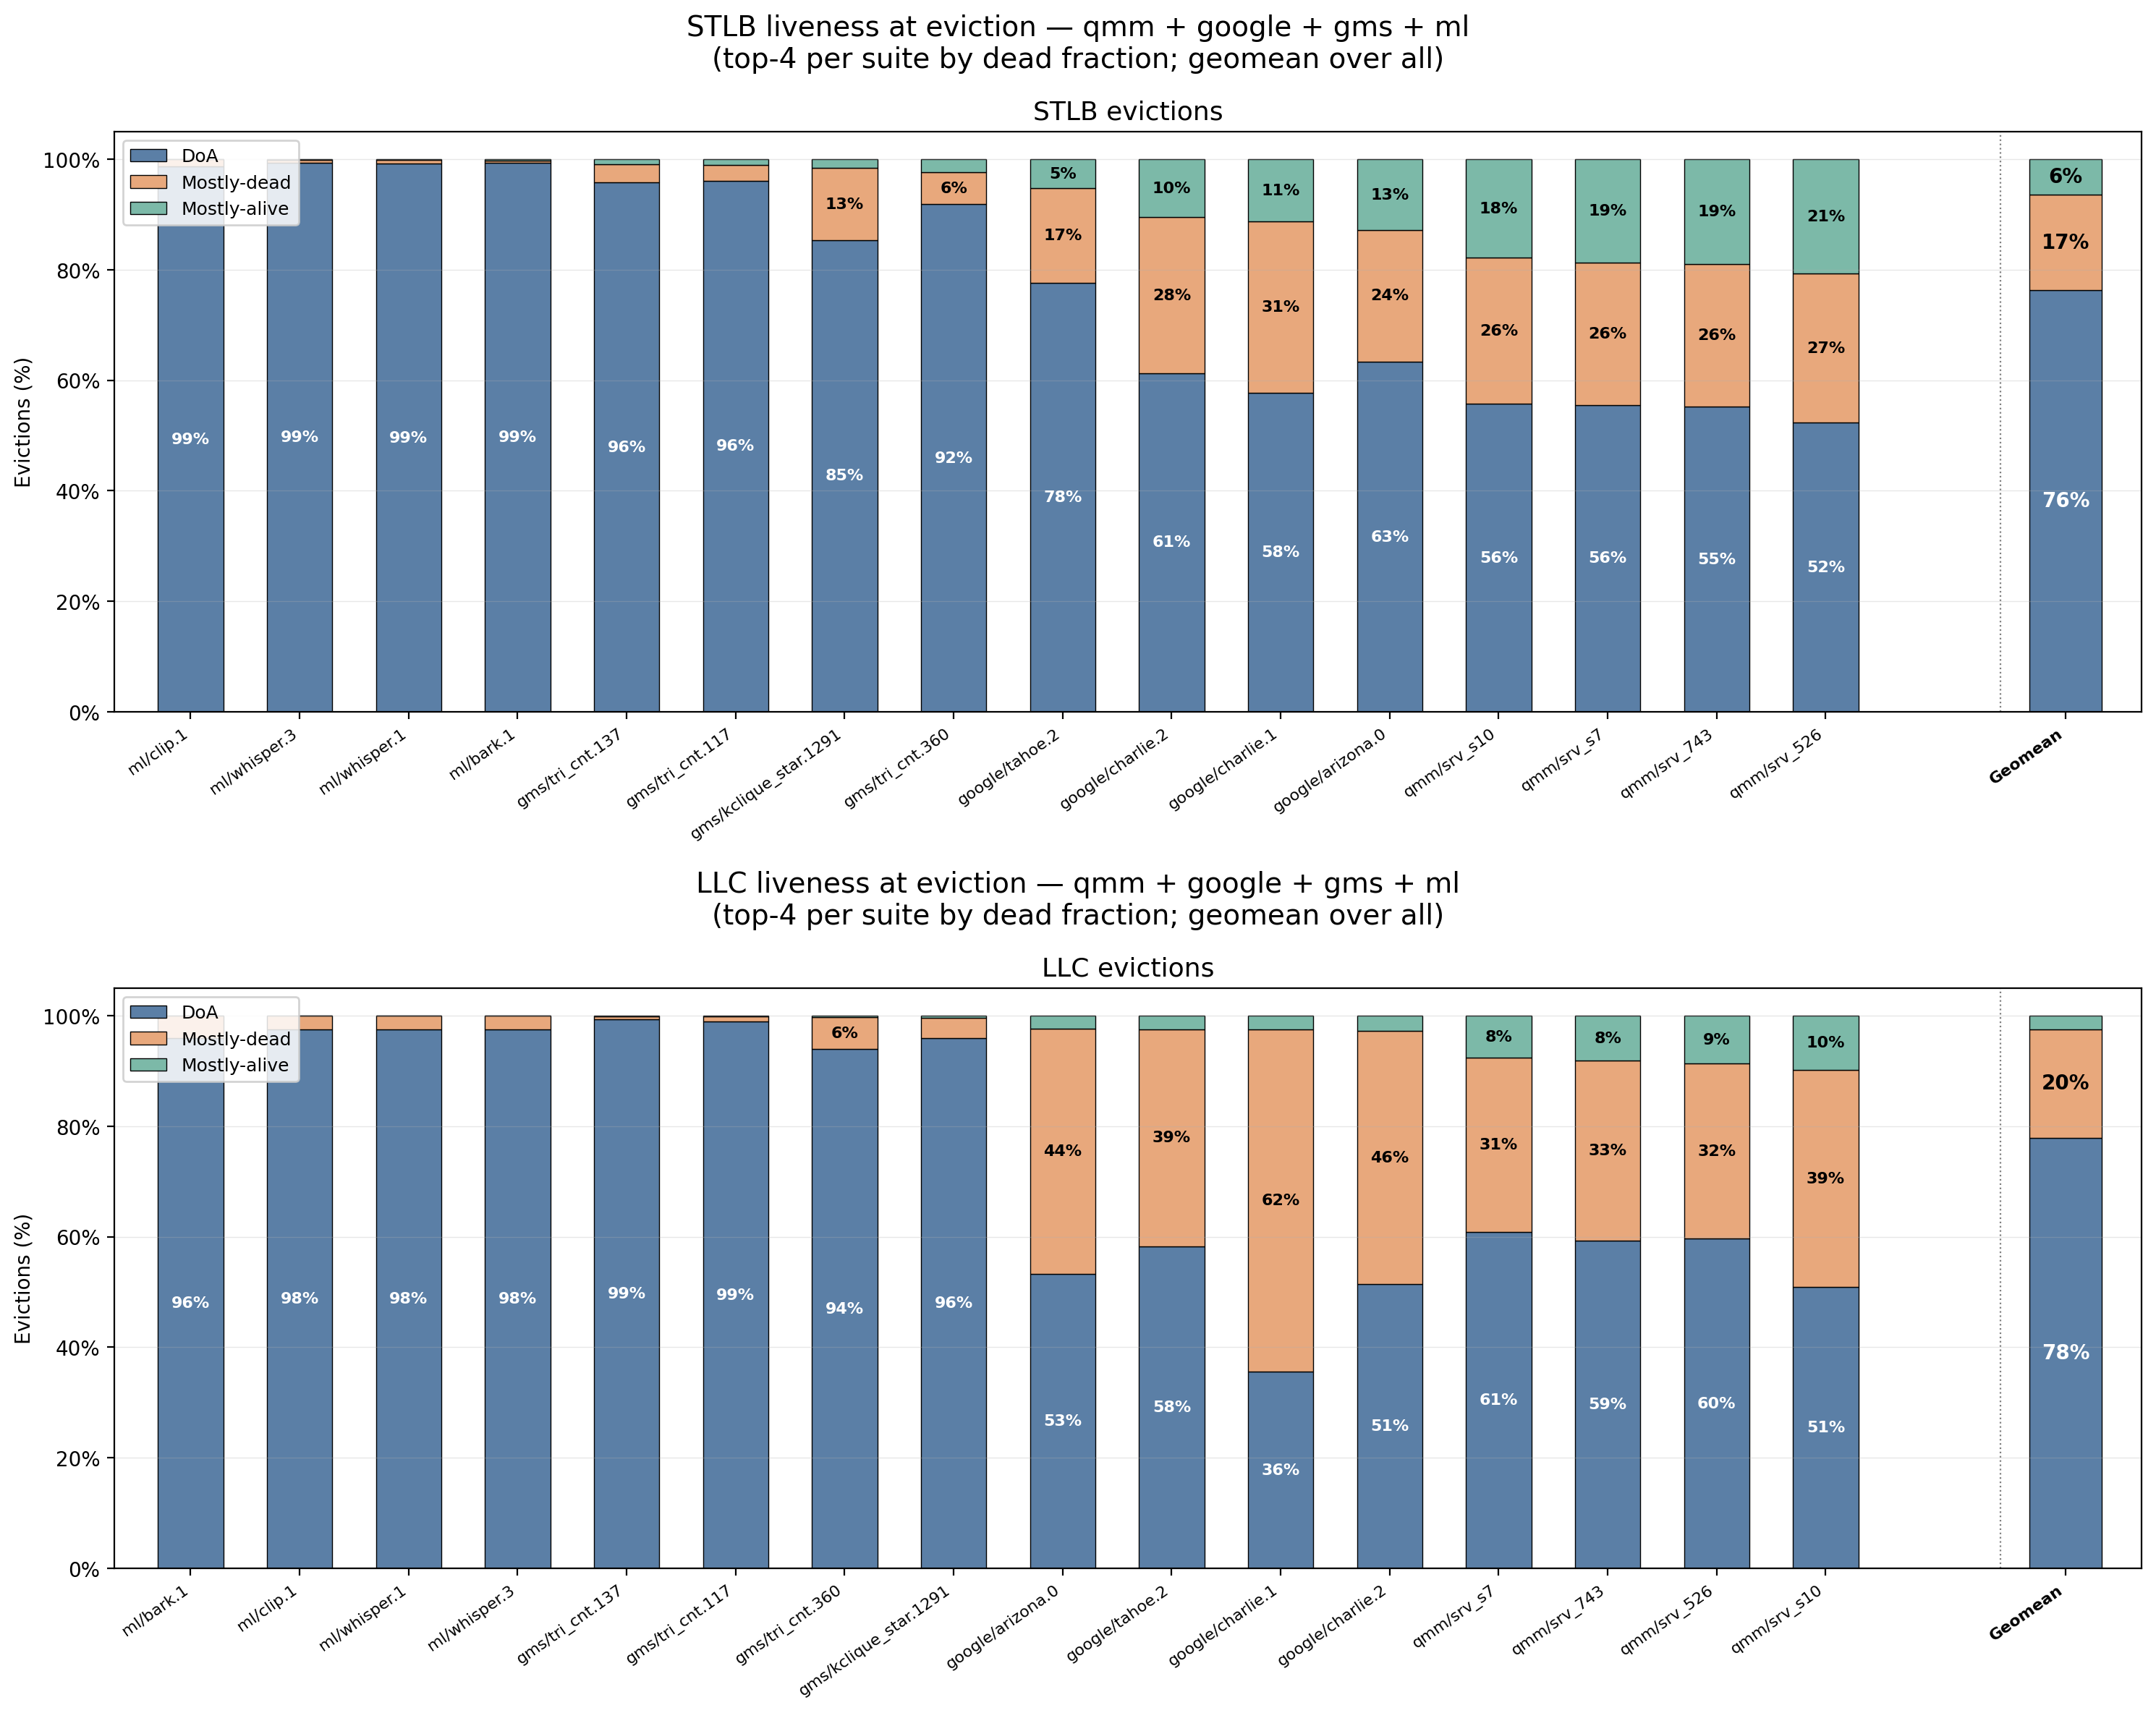
\includegraphics[width=\linewidth,height=0.55\textheight,keepaspectratio]{../../plots/liveness/new_liveness_bar_all.png}
  \caption{Per-workload liveness breakdown (STLB top, LLC bottom) for the
           new domains: Qualcomm, Google, GMS, and AI/ML.
           Each bar shows one workload (top-4 per suite by dead fraction);
           rightmost bar per suite is the geomean over all suite workloads.}
  \label{fig:liveness_bar_new}
\end{figure}

Figures~\ref{fig:liveness_bar_mazumdar} and \ref{fig:liveness_bar_new}
show that DoA and mostly-dead evictions together account for the large
majority of LLC traffic across all seven suites.
The basic premise for both mechanisms --- that substantial dead capacity
is wasted --- is well established regardless of workload class.
GAP and Ligra show high LLC DoA fractions consistent with their streaming
graph traversal patterns; AI/ML shows a bimodal structure reflecting the
mix of streaming model weights (uniformly dead) and hot KV-cache blocks
(mostly alive).

\subsection{LLC--STLB DoA Correlation}
\label{sec:correlation}

\begin{figure}[htbp]
  \centering
  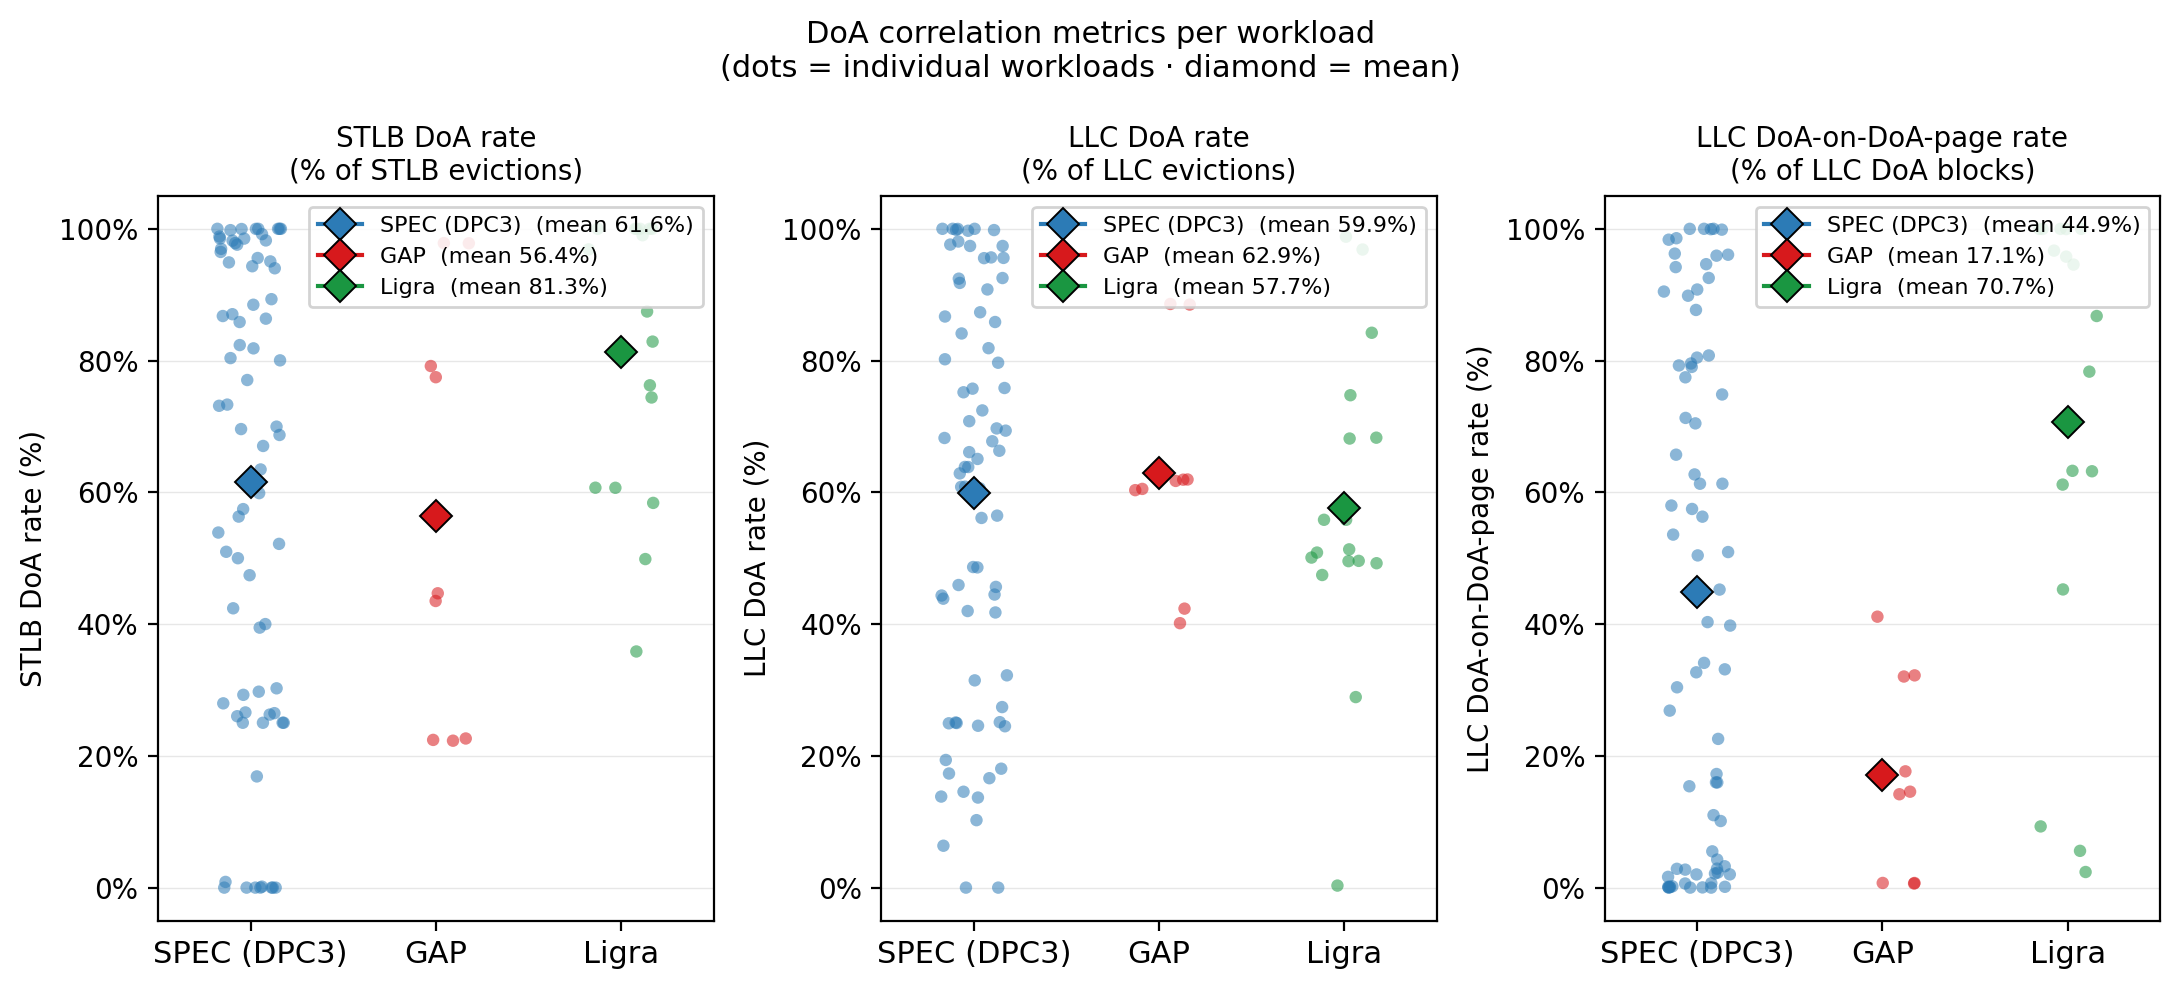
\includegraphics[width=\linewidth]{../../plots/liveness/mazumdar_liveness_corr_strip.png}
  \caption{LLC DoA rate, STLB DoA rate, and LLC--STLB DoA correlation
           for SPEC, GAP, and Ligra.}
  \label{fig:liveness_corr_mazumdar}
\end{figure}

\begin{figure}[htbp]
  \centering
  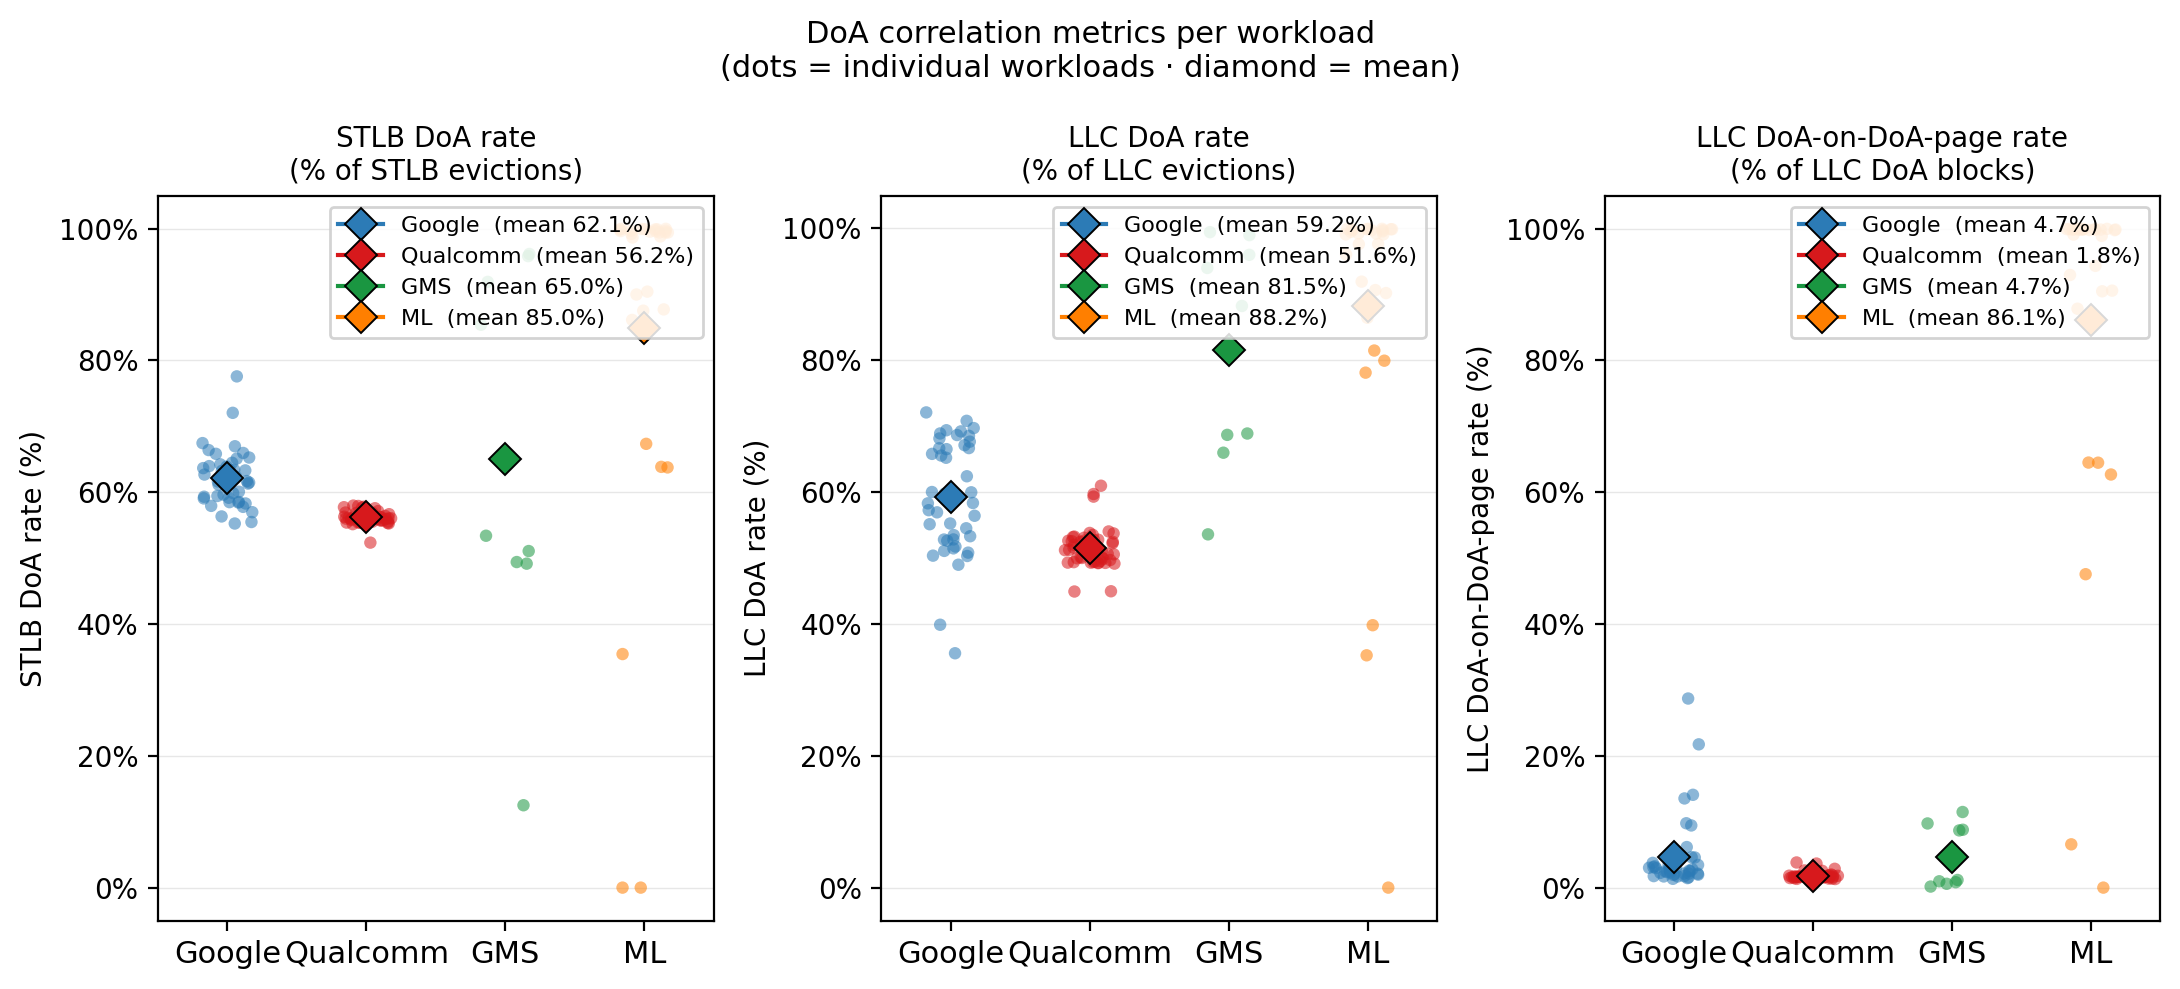
\includegraphics[width=\linewidth]{../../plots/liveness/new_suites_liveness_corr_strip.png}
  \caption{LLC DoA rate, STLB DoA rate, and LLC--STLB DoA correlation
           for Google, Qualcomm, GMS, and AI/ML.}
  \label{fig:liveness_corr_new}
\end{figure}

Figures~\ref{fig:liveness_corr_mazumdar} and \ref{fig:liveness_corr_new}
quantify how often a DoA LLC block sits on a page that the STLB also
classifies as DoA.
The results fall into three groups.

\emph{Moderate correlation --- SPEC (${\sim}33\%$) and GMS (${\sim}9\%$).}
Roughly one-third of SPEC's DoA LLC evictions map to a DoA STLB page,
giving dpPred useful signal.
GMS is intermediate: enough structure for a modest predictor gain, but
far below SPEC.

\emph{Near-zero correlation --- Google (${\sim}4\%$), Qualcomm (${\sim}2\%$), and GAP (${\sim}1\%$).}
Server workloads densely pack live and dead blocks onto the same pages;
GAP's graph frontier has fine-grained per-block liveness that the coarser
page-level signal cannot resolve.
In all three cases the STLB DoA signal is almost entirely decoupled from
LLC DoA, leaving dpPred without actionable signal.

\emph{Very high correlation --- Ligra and AI/ML (${\sim}100\%$).}
Streaming graph kernels (Ligra) and large model-weight operands (AI/ML)
exhibit such uniform access patterns that dead LLC blocks are
overwhelmingly concentrated on pages that are also DoA in the STLB.
This is precisely the hypothesis from Mazumdar~2021 confirmed
empirically: when a workload's streaming operands occupy entire pages
without mixing with live data, the page-level signal becomes highly
predictive of block-level liveness.

This correlation is the single most important number for predicting
bypass predictor effectiveness: high correlation means the STLB can
identify which pages to bypass; near-zero correlation means it cannot.

\subsection{Bypass Predictor Performance}
\label{sec:bypass_perf}

dpPred maintains a PC-indexed page-history table that tracks how often
each faulting PC produces pages whose STLB Accessed bit is clear at check
time.
When the counter exceeds a confidence threshold \texttt{pconf}, the page
frame number (PFN) is pushed into the Page Frame Queue (PFQ, capacity~8).
cbPred then gates LLC bypass on PFQ membership plus a block-level counter
(\texttt{bconf}).
Full mechanism details are in Section~\ref{sec:bypass}.

\begin{figure}[htbp]
  \centering
  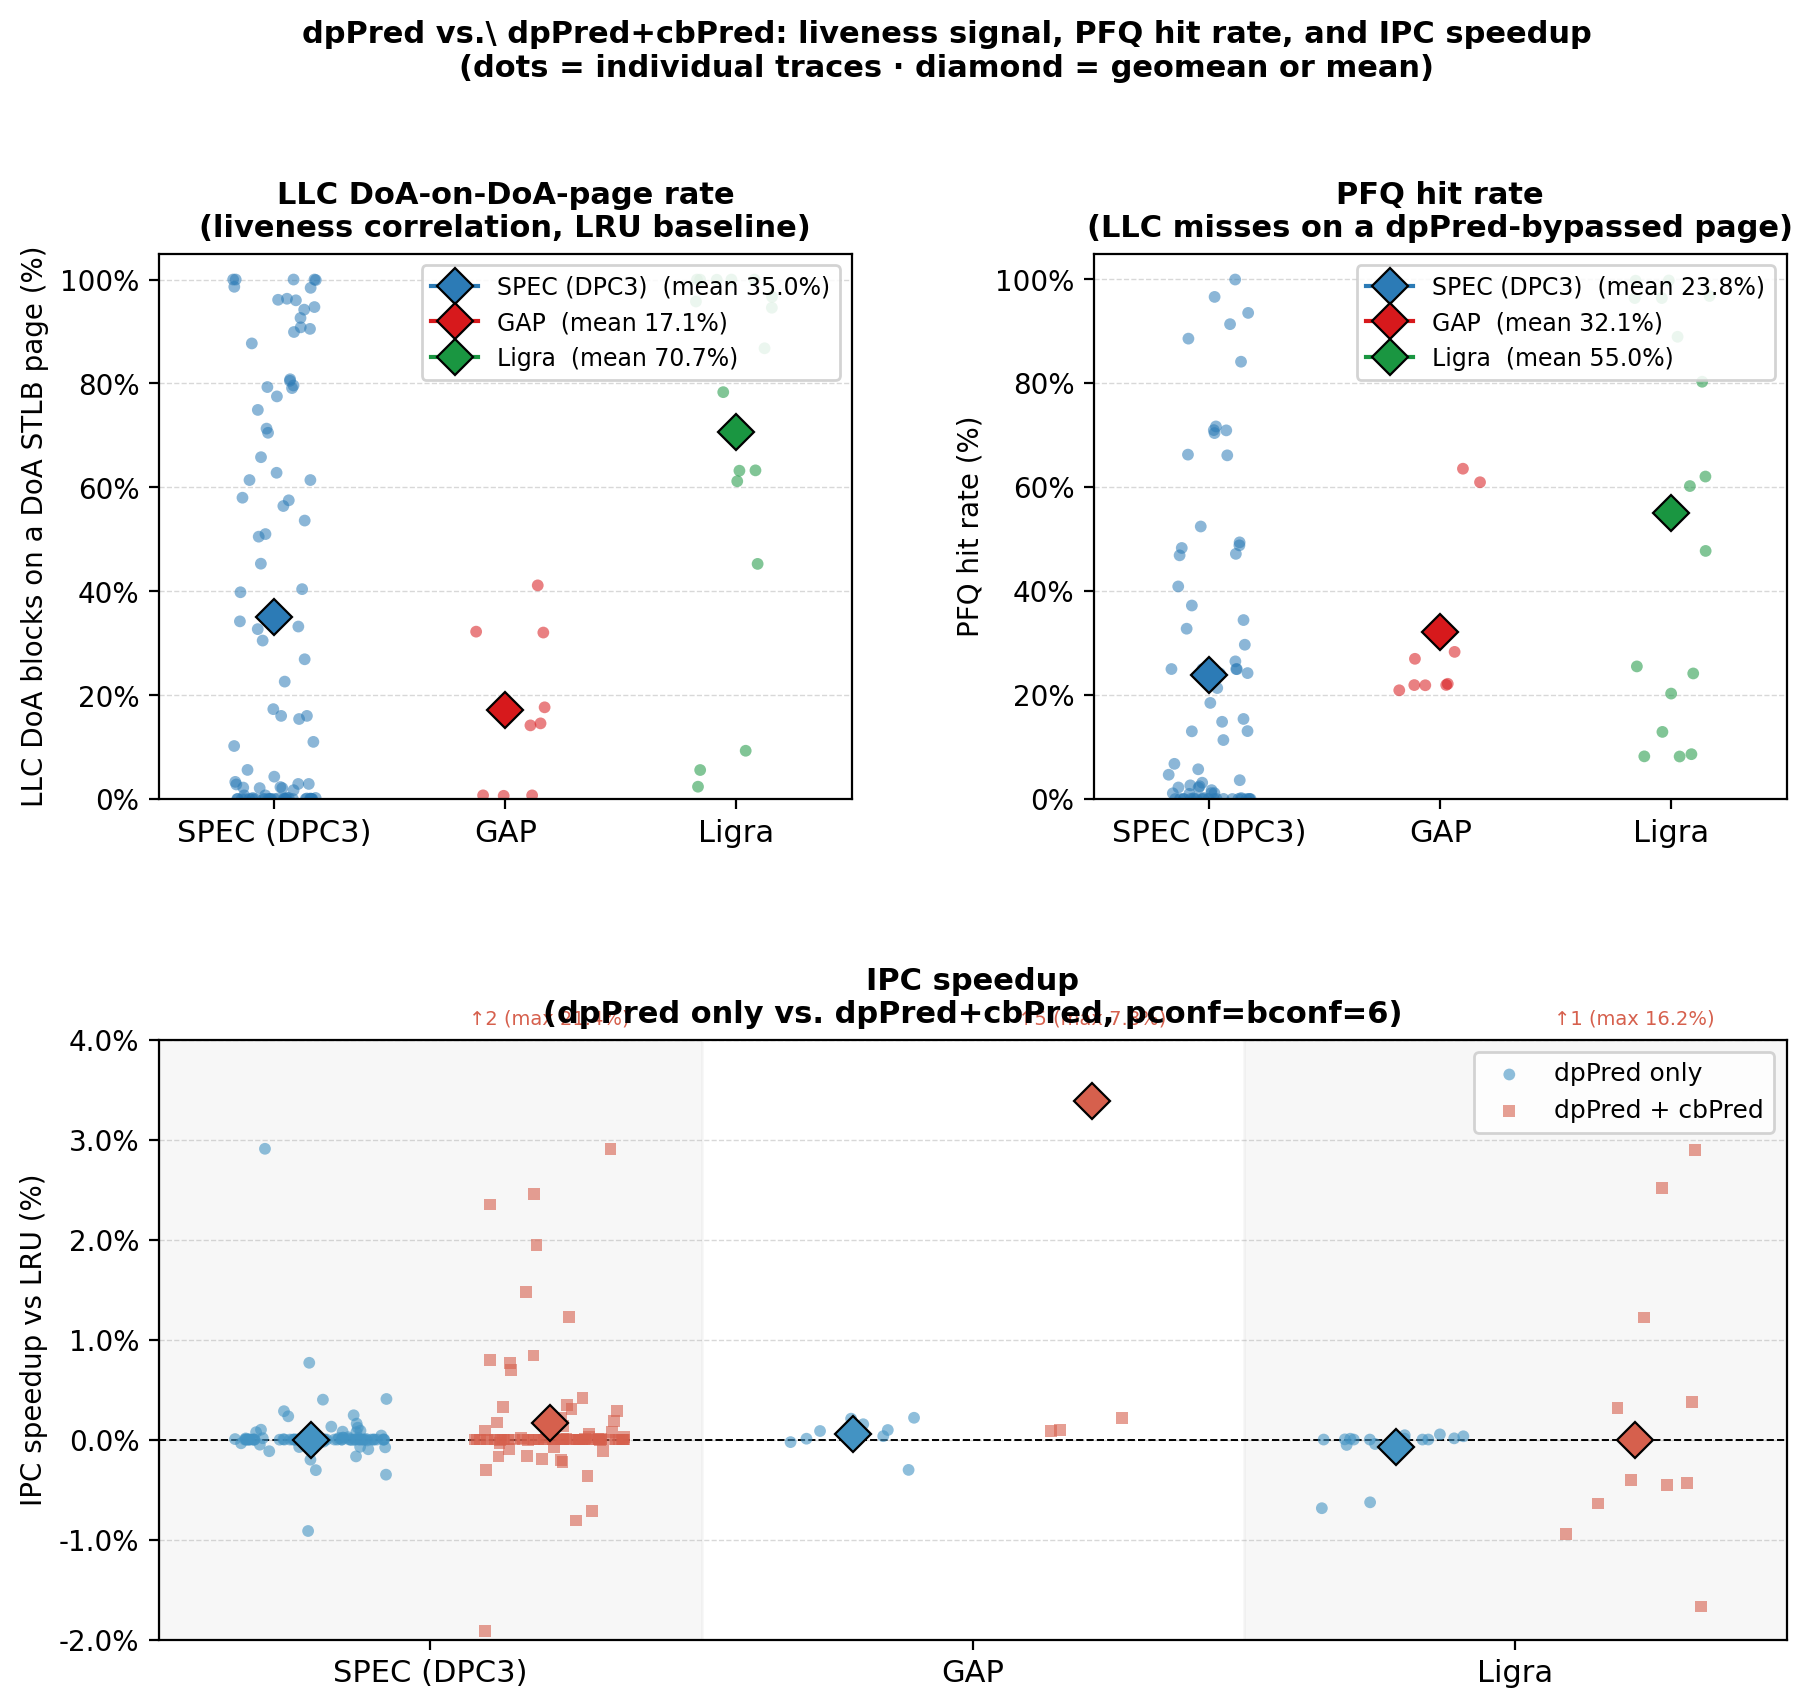
\includegraphics[width=\linewidth]{../../plots/predictor/mazumdar_predictor/speedup_pfq_correlation.png}
  \caption{Predictor study for SPEC, GAP, and Ligra.
           Top left: LLC DoA-on-DoA-STLB-page rate.
           Top right: PFQ hit rate.
           Bottom: IPC speedup vs.\ LRU for dpPred only and dpPred+cbPred
           at pconf\,=\,bconf\,=\,6.
           Dots: individual traces; diamonds: geomeans.}
  \label{fig:bypass_pred_mazumdar}
\end{figure}

\begin{figure}[htbp]
  \centering
  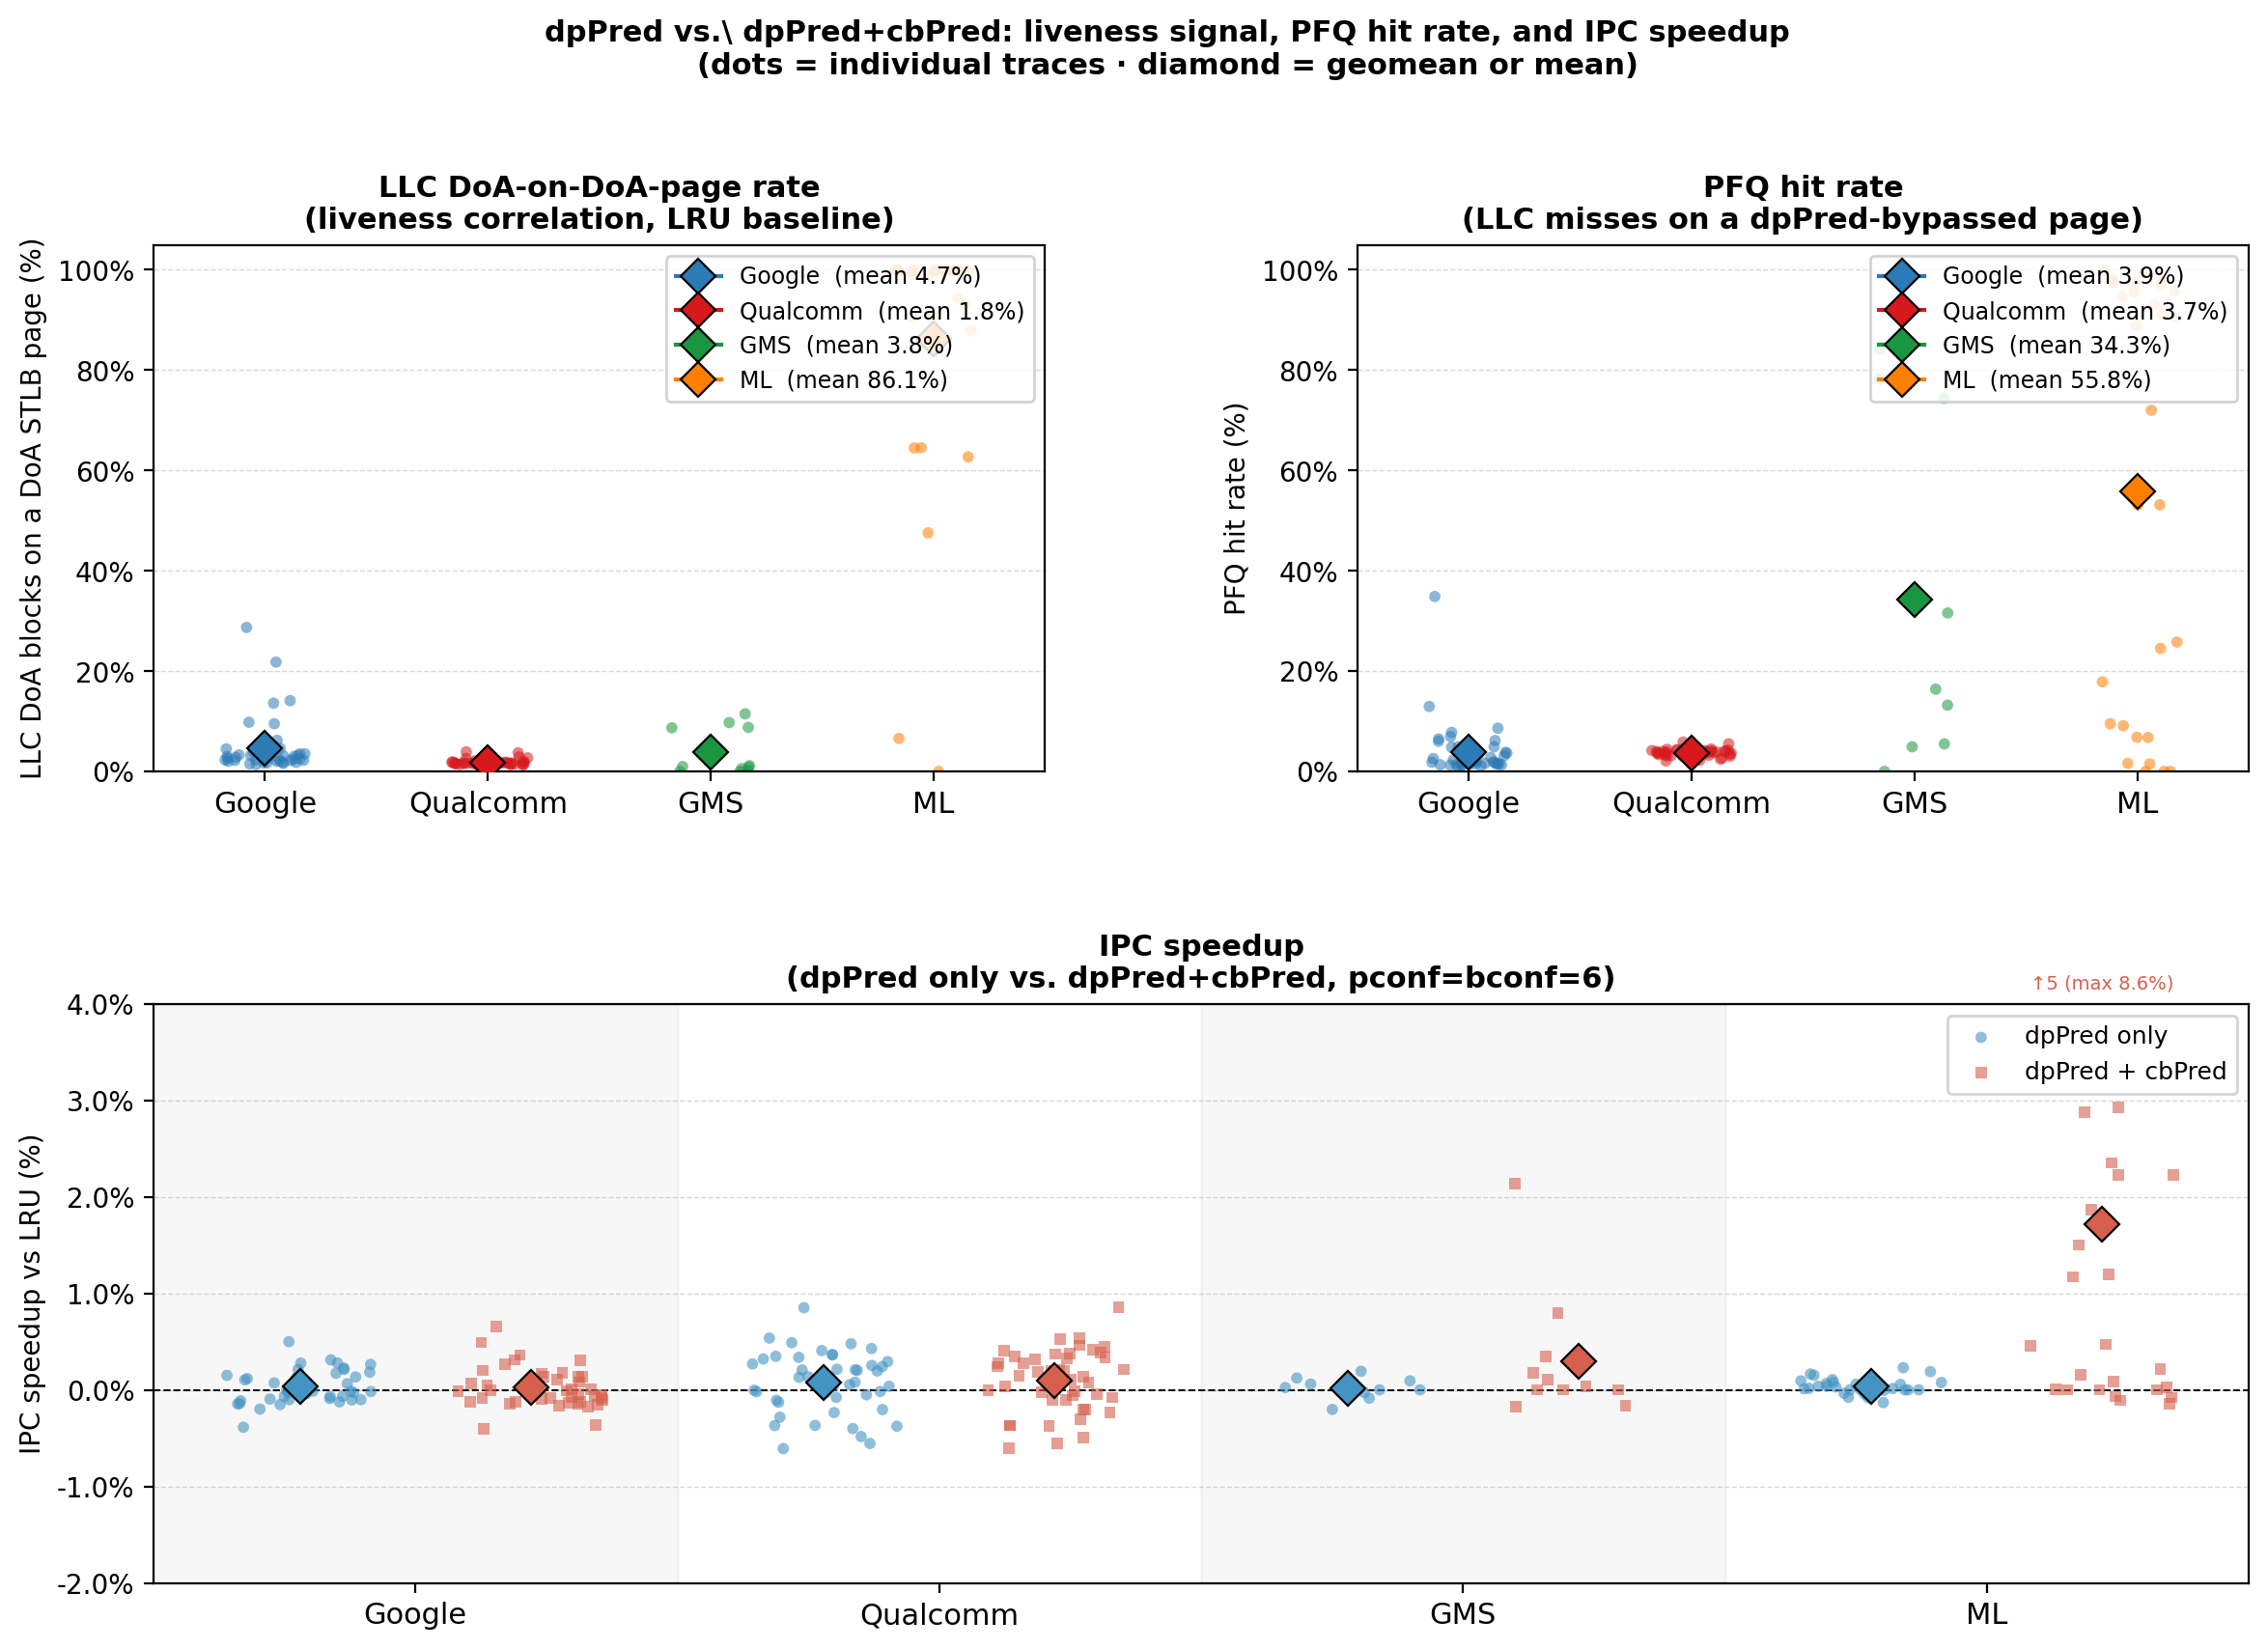
\includegraphics[width=\linewidth]{../../plots/predictor/new_suites_predictor/speedup_pfq_correlation.png}
  \caption{Predictor study for Google, Qualcomm, GMS, and AI/ML.
           Same layout as Figure~\ref{fig:bypass_pred_mazumdar}.}
  \label{fig:bypass_pred_new}
\end{figure}

Figures~\ref{fig:bypass_pred_mazumdar} and \ref{fig:bypass_pred_new}
confirm the prediction from Section~\ref{sec:correlation}: dpPred gains
track the DoA correlation closely across all seven suites.
On SPEC, a ${\sim}33\%$ correlation produces a consistent if modest
speedup.
GAP's near-zero correlation (${\sim}1\%$) makes dpPred ineffective there
despite high LLC DoA rates, mirroring the server workload pattern.
Ligra's near-perfect correlation (${\sim}100\%$) makes it the clearest
beneficiary: the predictor can almost always identify DoA pages.
Google and Qualcomm remain near-zero as expected.
GMS falls between SPEC and server.
AI/ML's very high correlation similarly suggests dpPred has strong signal
there.

Note that dpPred-only operates exclusively at the STLB: it records which
pages are predicted DoA but does not yet alter LLC behaviour.
The IPC gain at this stage is entirely from STLB policy changes
(bypassing page-table walks for predicted-DoA pages).

The top-right panels show the PFQ hit rate: the fraction of LLC fills
whose PFN was in the PFQ.
This rate tracks the DoA correlation closely across all suites.
On SPEC (correlation ${\sim}33\%$) cbPred adds a consistent positive
margin over dpPred alone; on Google and Qualcomm (correlation
${\sim}2$--$4\%$) the marginal gain from cbPred is negligible.
Ligra and AI/ML, with near-perfect correlation, have the highest PFQ
hit rates and consequently the largest cbPred margins.
GAP, despite high LLC DoA rates, shows a low PFQ hit rate consistent
with its near-zero correlation --- the PFQ is rarely populated with
the right PFN.

The double-gate structure caps cbPred's coverage at the PFQ hit rate,
which in turn is bounded by the DoA correlation.
On mixed-liveness workloads (server, GAP) most DoA LLC blocks are
inserted regardless of their block-level confidence.
Relaxing the gate is explored in Section~\ref{sec:bconf_only}.

% ─────────────────────────────────────────────────────────────────────────────
\section{Liveness-Guided Replacement Policy}
\label{sec:replacement}
% ─────────────────────────────────────────────────────────────────────────────

\subsection{srrip\_live: block-level liveness at insertion}

\texttt{srrip\_live} extends SRRIP by setting the initial RRPV of each
block based on the liveness class observed the last time the same PC
filled the LLC.
Blocks from PCs with a predominantly dead fill history are inserted with a
high RRPV (evict soon); blocks from PCs with a live history are inserted
with a low RRPV (keep longer).
The key property distinguishing this from the bypass predictor is
granularity: liveness is tracked per PC at the LLC-block level, not per PC
at the page level.
Individual blocks on a mixed-liveness page can therefore be classified
independently --- the signal that was lost at the STLB level is
recoverable at the LLC level.

\subsection{LLC-only: threshold sensitivity and indexing}

\begin{figure}[htbp]
  \centering
  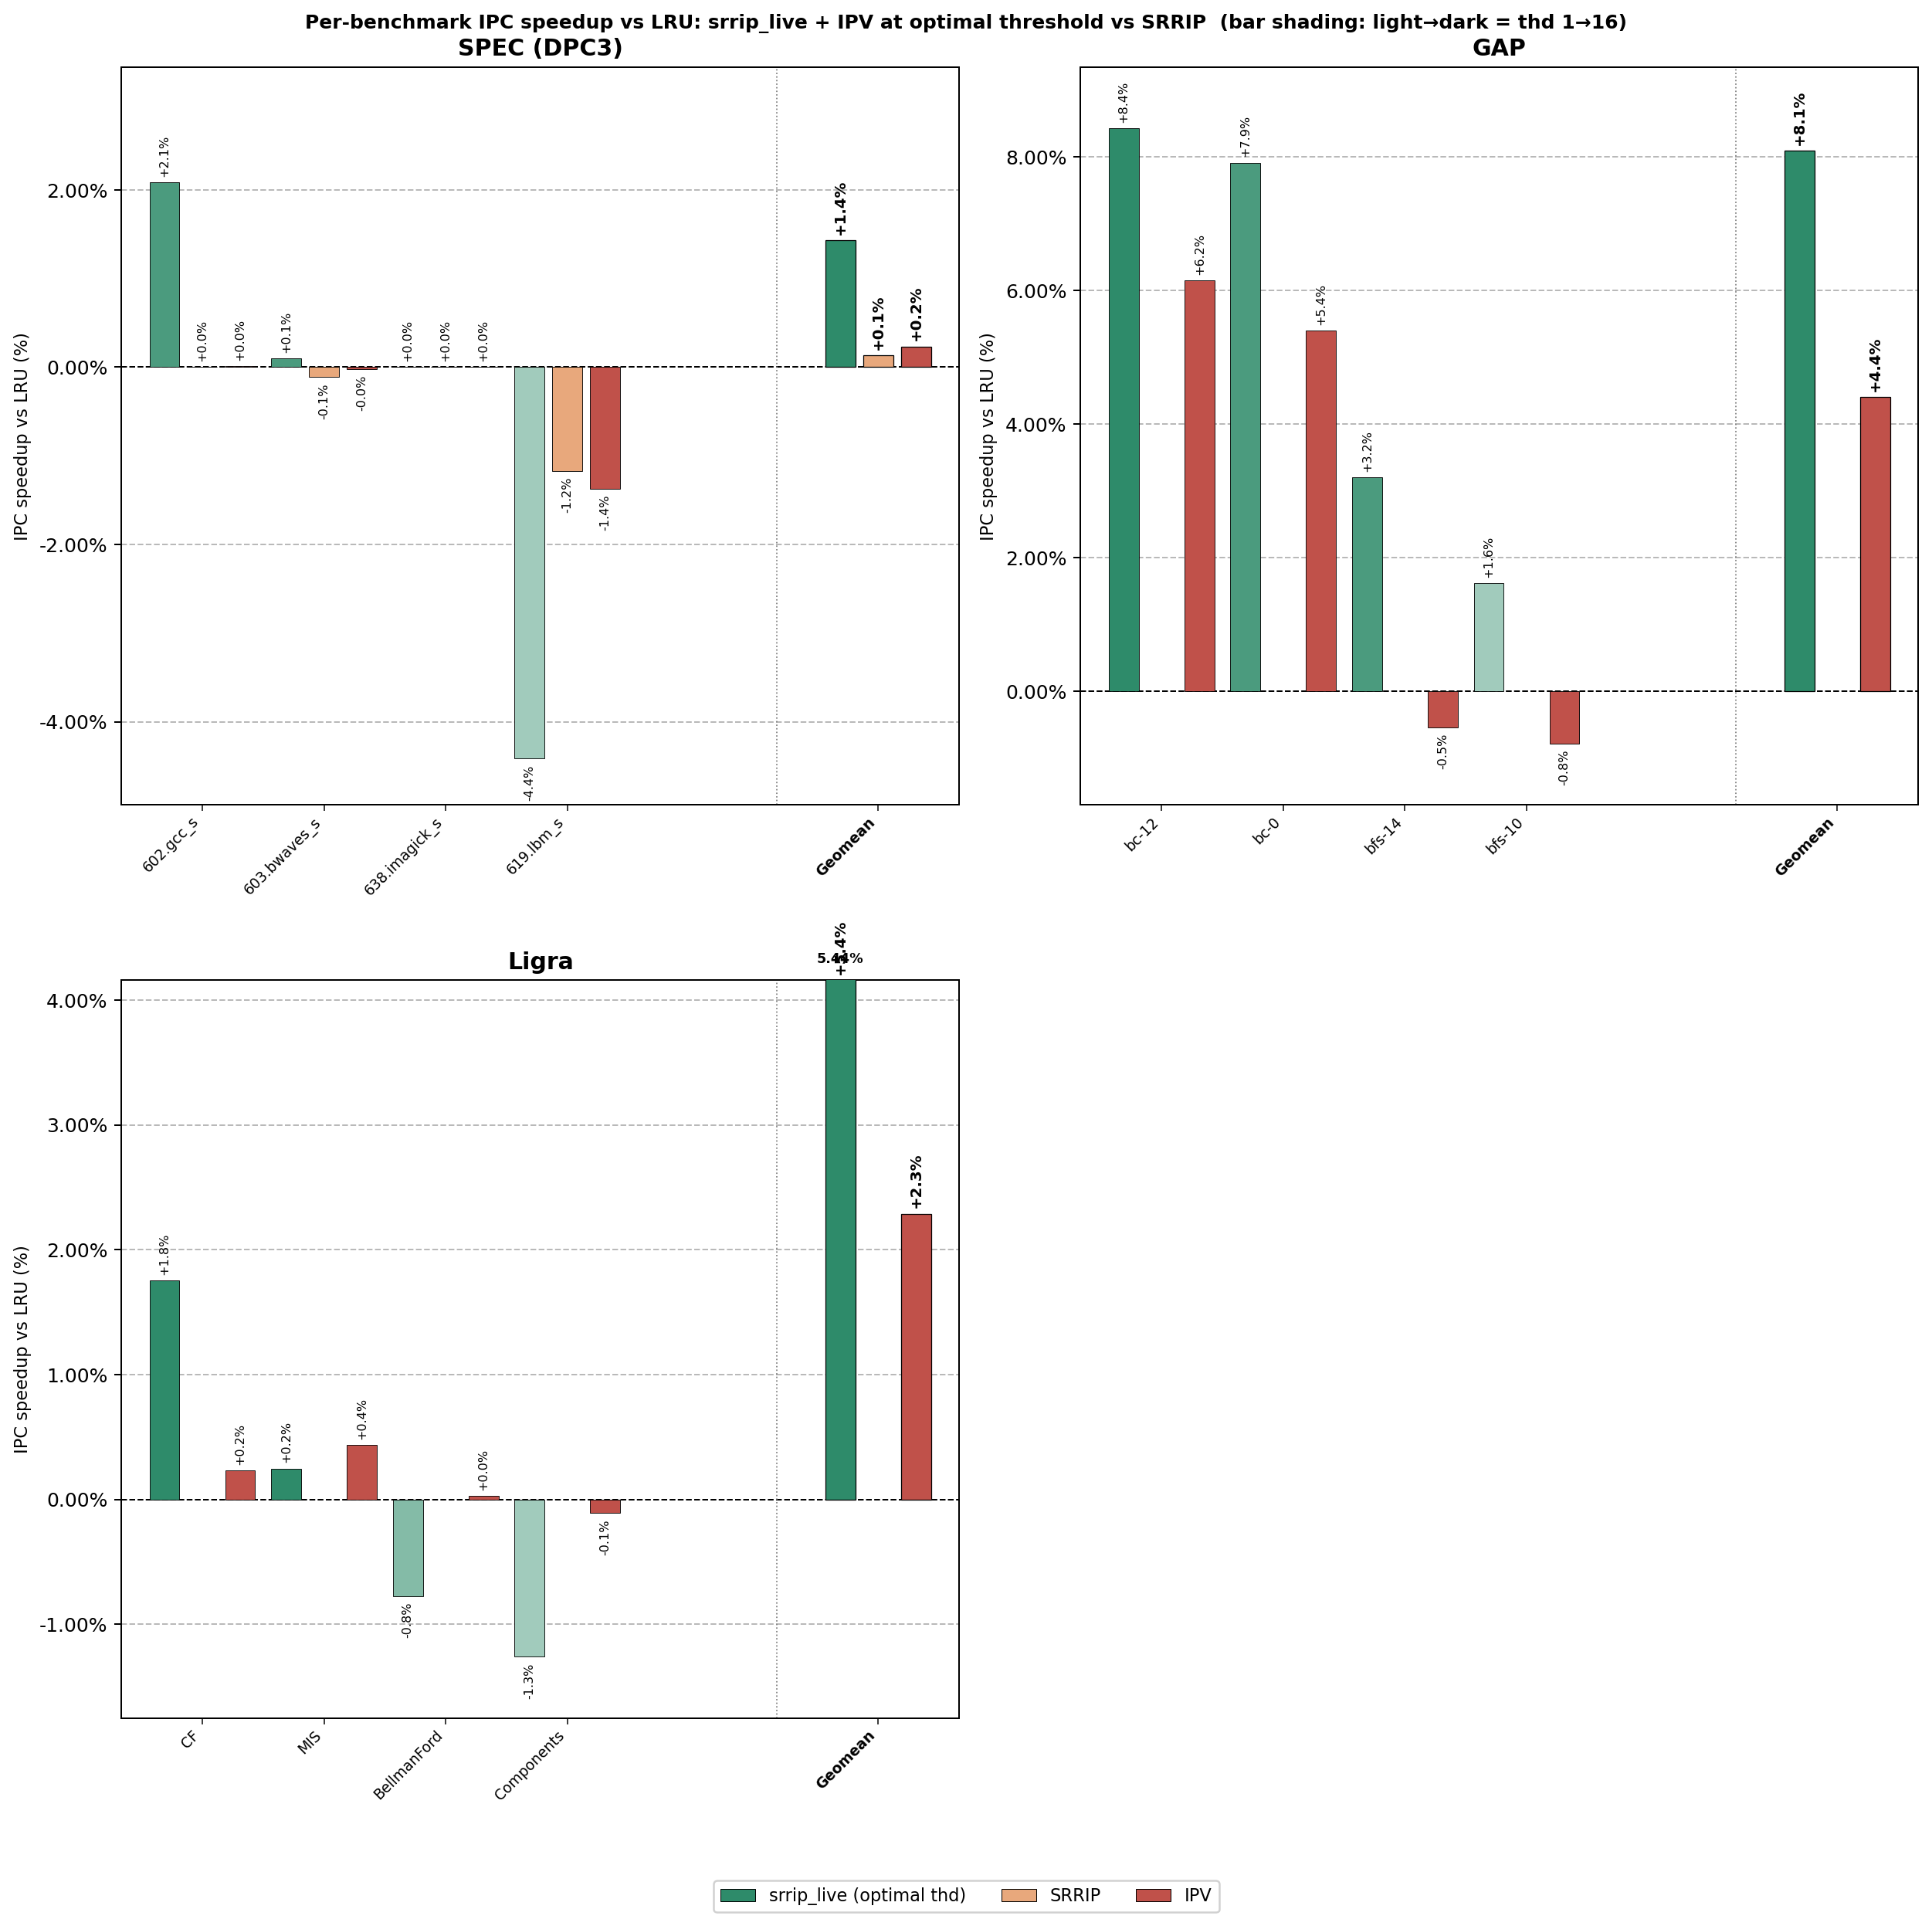
\includegraphics[width=\linewidth]{../../plots/optimal_thd_maz_pc.png}
  \caption{Per-workload IPC speedup vs.\ LRU for \texttt{srrip\_live}
           at each workload's individually optimal mid\_thd (PC-indexed
           history) for SPEC, GAP, and Ligra.
           Four workloads per suite (top-4 by dead fraction) plus suite geomean.
           Bar shading (light~$\to$~dark) = threshold $1 \to 16$.
           SRRIP bars shown for reference.}
  \label{fig:srrip_live_thd}
\end{figure}

\begin{figure}[htbp]
  \centering
  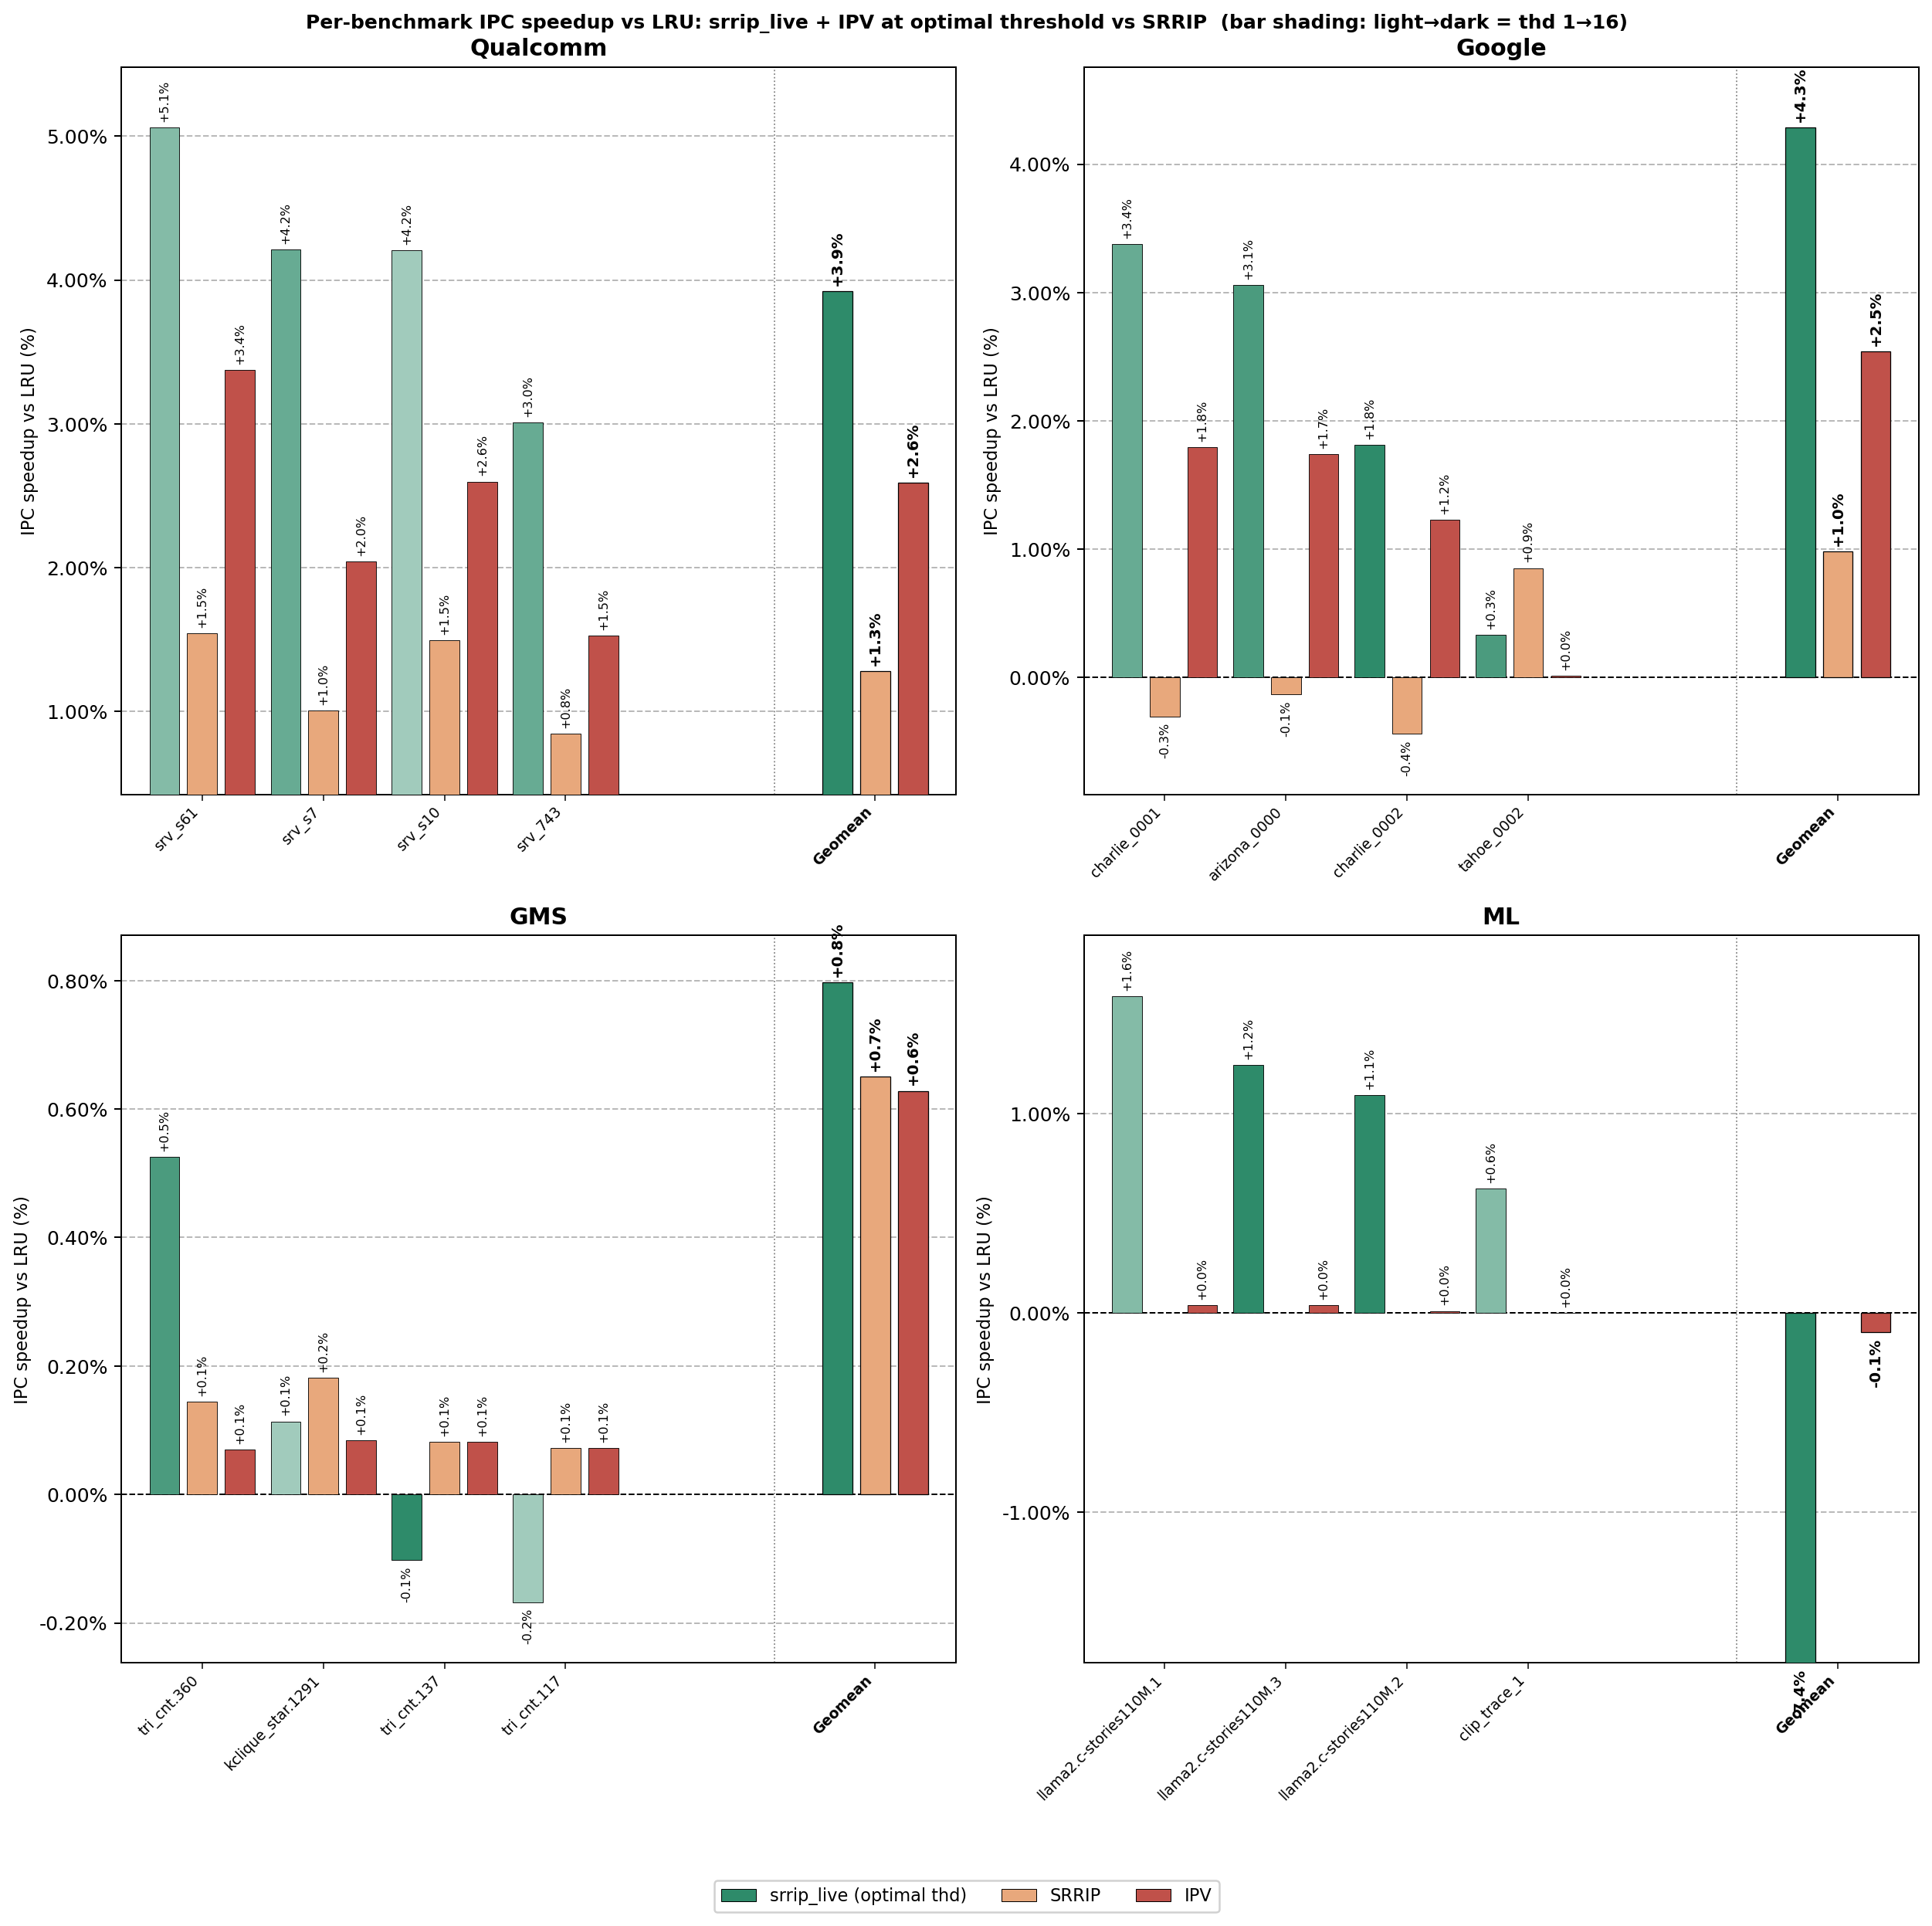
\includegraphics[width=\linewidth]{../../plots/optimal_thd_new_pc.png}
  \caption{As Figure~\ref{fig:srrip_live_thd} for Qualcomm, Google, GMS,
           and AI/ML.}
  \label{fig:srrip_live_thd_new}
\end{figure}

Figures~\ref{fig:srrip_live_thd} and~\ref{fig:srrip_live_thd_new} show each workload at its individually
optimal threshold, revealing the within-suite variance that suite geomeans
would obscure.
SPEC is the most heterogeneous: \texttt{605.mcf\_s} gains $+16.6\%$
while \texttt{619.lbm\_s} loses $-4.4\%$, both at their respective
optimal thresholds.
Server suites (Qualcomm, Google) are consistently positive and
tightly clustered, reflecting uniform fleet workload profiles.
Graph suites (GAP, Ligra) show a range from small gains to large ones;
GAP frontier-access traces benefit strongly.
GMS shows only modest gains throughout.
AI/ML is the clearest failure case: with PC-indexed history, several
traces are substantially hurt regardless of threshold.
Address-indexed history resolves this
(Figure~\ref{fig:srrip_live_thd_addr}), recovering near-neutral or
positive speedup across all AI/ML workloads.

\textit{SPEC.}
Benchmarks with highly concentrated, predictable access streams benefit
the most: \texttt{605.mcf\_s} (sparse graph traversal) gains
$+16.6\%$, far above its SRRIP baseline of $+2.6\%$, because a small
number of load PCs dominate dead insertions.
\texttt{623.xalancbmk\_s} (XML transform) and \texttt{627.cam4\_s}
(atmospheric model) also gain substantially while SRRIP is neutral or
slightly harmful --- liveness history assigns high initial RRPV to blocks
that SRRIP would treat identically to live ones.
Streaming kernels are the counter-case: \texttt{619.lbm\_s} (lattice
Boltzmann) is hurt ($-4.4\%$), because its access pattern changes over
time and the per-PC liveness history built in warmup misleads the policy
during simulation.
\texttt{607.cactuBSSN\_s} (astrophysics PDE solver) is also hurt for
similar reasons.
\texttt{620.omnetpp\_s} (network simulation) is the one SPEC benchmark
where plain SRRIP outperforms \texttt{srrip\_live}: the mid-RRPV
heuristic happens to match its access pattern without needing per-PC
history.

\textit{Server workloads.}
A notable feature of both server suites is their low inter-trace variance:
individual Google workloads span only $+0.3\%$ to $+8.5\%$ and Qualcomm
workloads span $+2.8\%$ to $+5.2\%$, so a small representative sample
captures the suite behaviour accurately.
This uniformity reflects the shared infrastructure and access patterns
within each fleet.
All server traces gain with \texttt{srrip\_live} despite the near-zero
LLC--STLB DoA correlation, confirming that block-level liveness is
recoverable even when the page-level signal is absent.
SRRIP is consistently near zero or slightly negative for Google and
Qualcomm: its uniform mid-RRPV assignment cannot exploit the per-PC
liveness skew that \texttt{srrip\_live} captures.

\textit{Graph suites.}
GAP graph-traversal workloads gain strongly (geomean $+7.9\%$) because
frontier access PCs are persistently dead and the history table classifies
them quickly.
Ligra graph-computing workloads show wide per-trace variance: some
streaming kernels (e.g.\ Triangle) gain $+33.9\%$, while others gain
only $+1$--$2\%$.
GMS graph-mining workloads show modest gains (under $+1\%$), consistent
with short, compute-intensive kernels leaving little room for replacement
policy differentiation.
AI/ML is a failure case for PC-indexed history on several traces
(bark.cpp.5 $-69\%$, stable-diffusion $-60\%$): non-stationary
PC-liveness patterns cause the history table to give misleading guidance.
Address-indexed history resolves this (see Figure~\ref{fig:srrip_live_thd_addr}).

No single threshold is universally optimal across workloads (shading
varies), confirming the need for per-suite threshold tuning.

\begin{figure}[htbp]
  \centering
  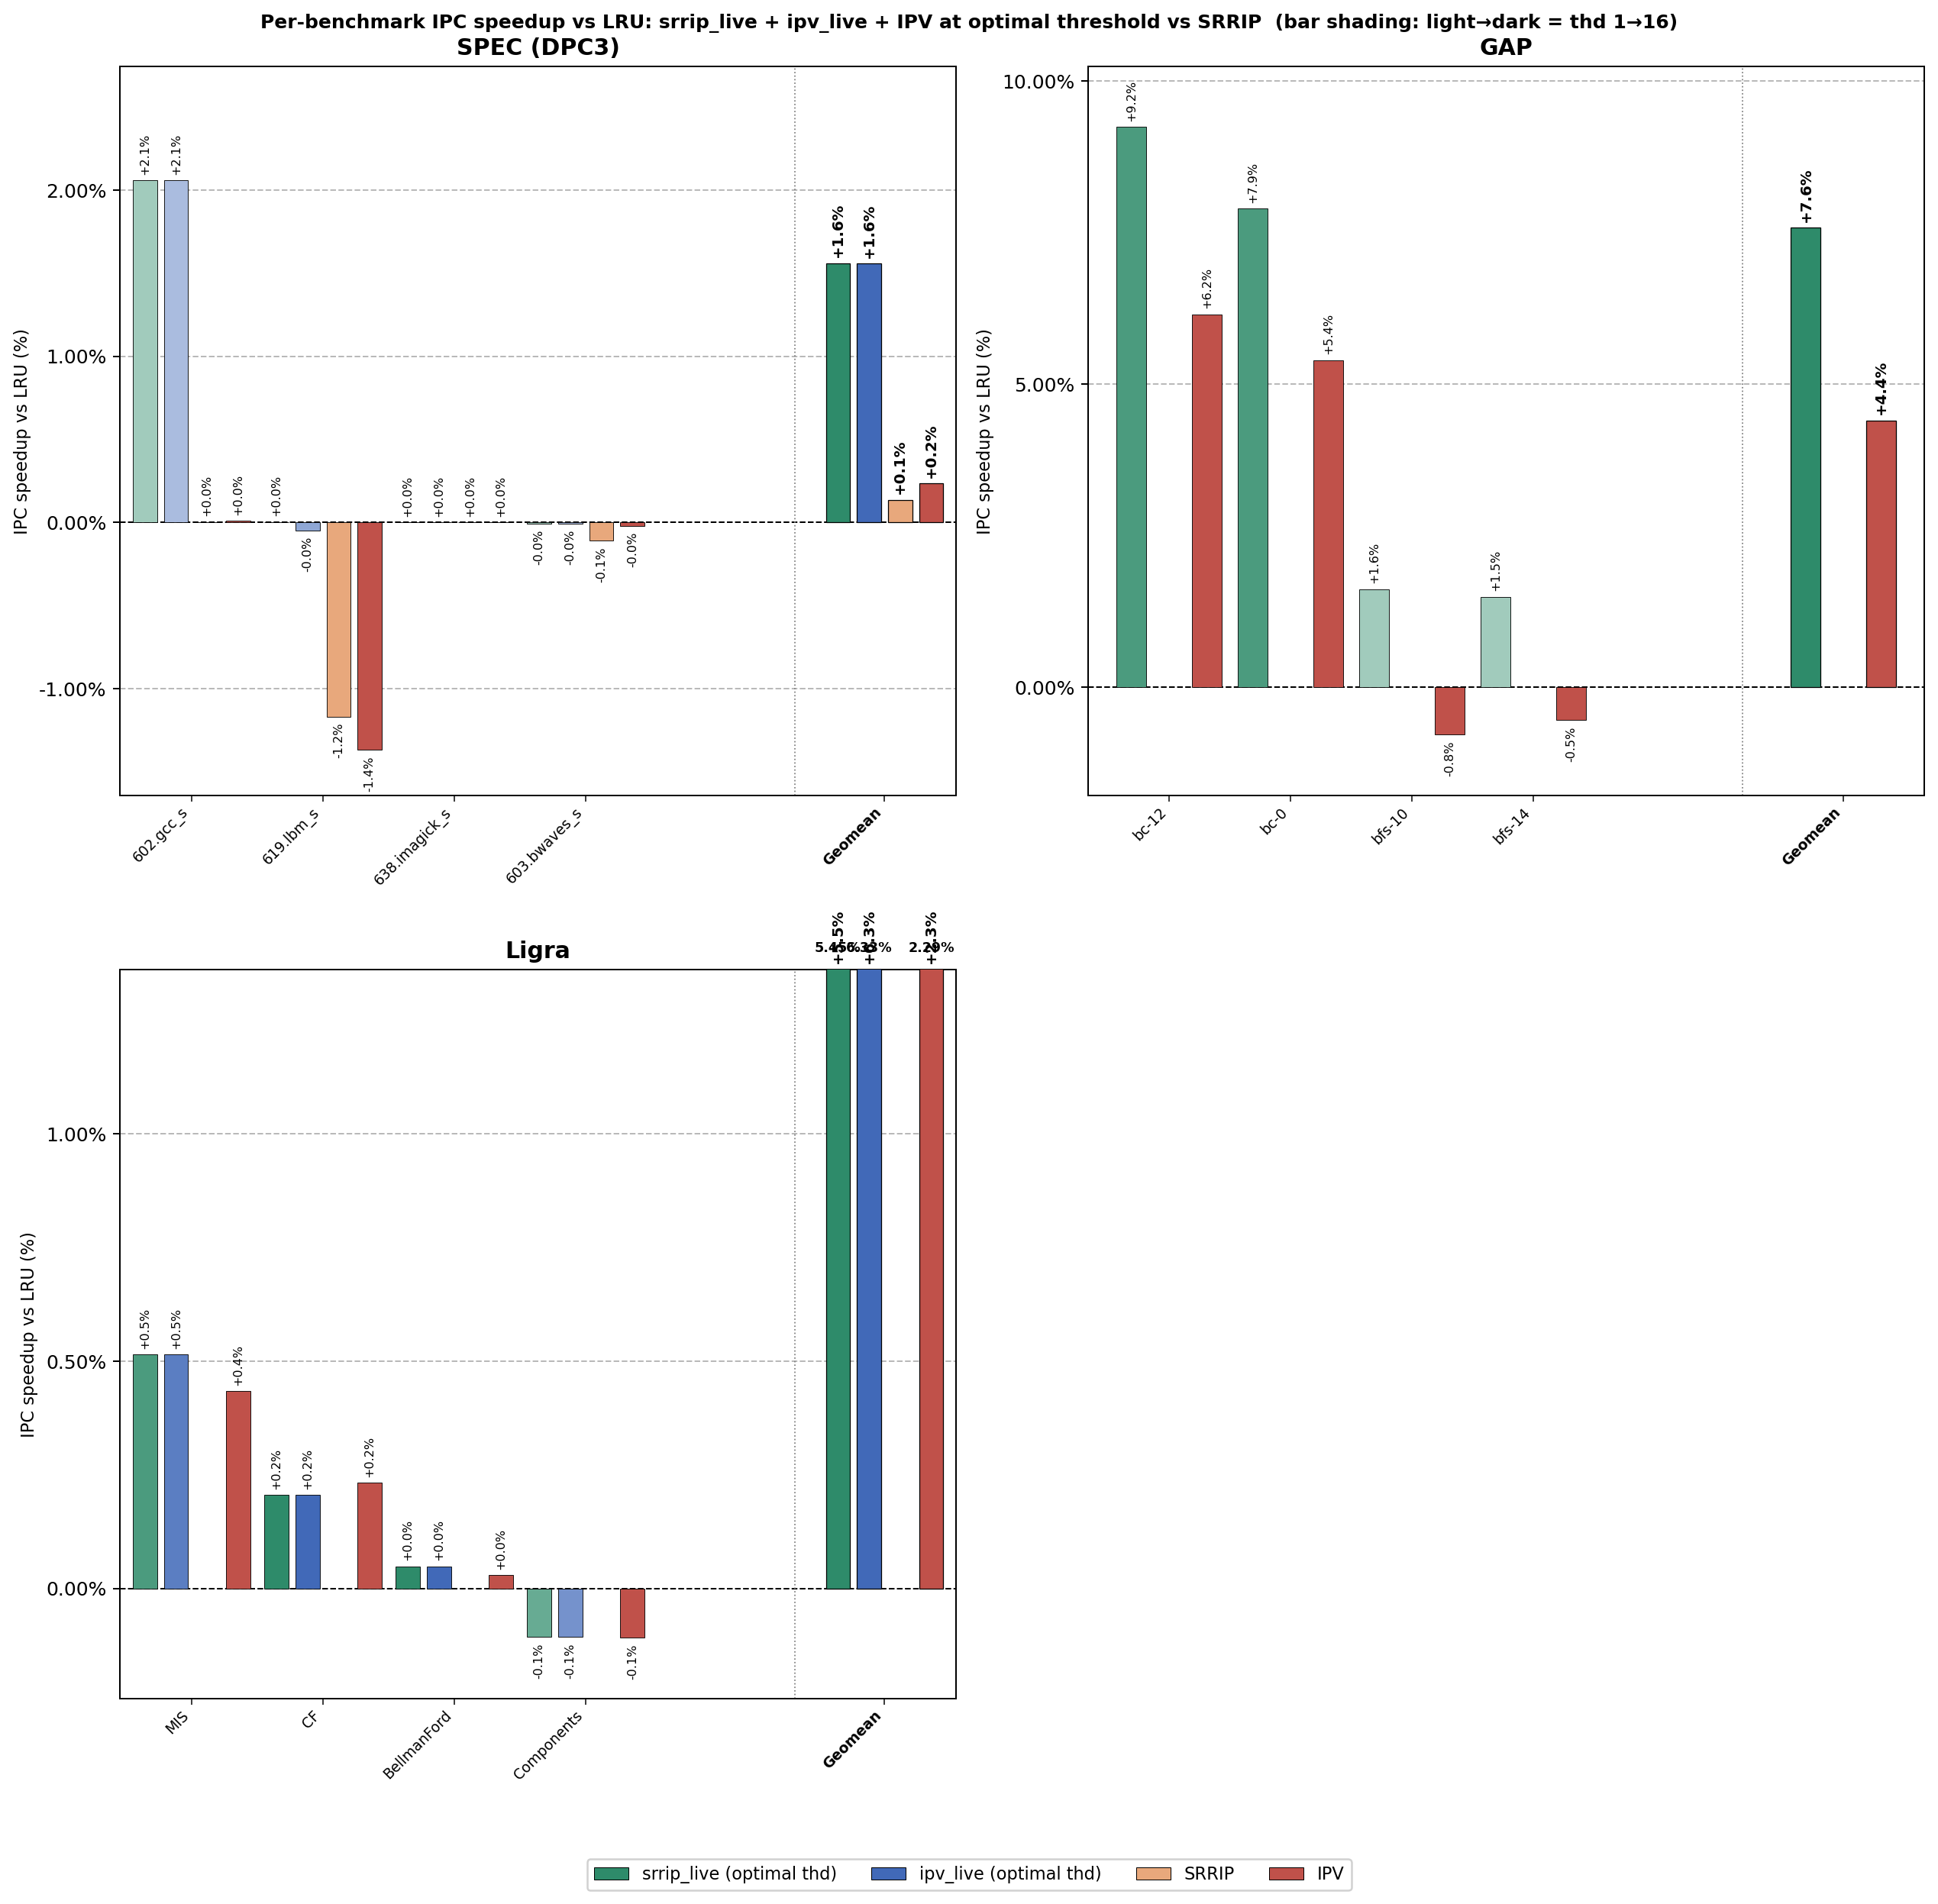
\includegraphics[width=\linewidth]{../../plots/optimal_thd_maz_addr.png}
  \caption{Address-indexed history --- per-workload IPC speedup vs.\ LRU
           for \texttt{srrip\_live} at each workload's individually optimal
           mid\_thd, for SPEC, GAP, and Ligra.}
  \label{fig:srrip_live_thd_addr}
\end{figure}

\begin{figure}[htbp]
  \centering
  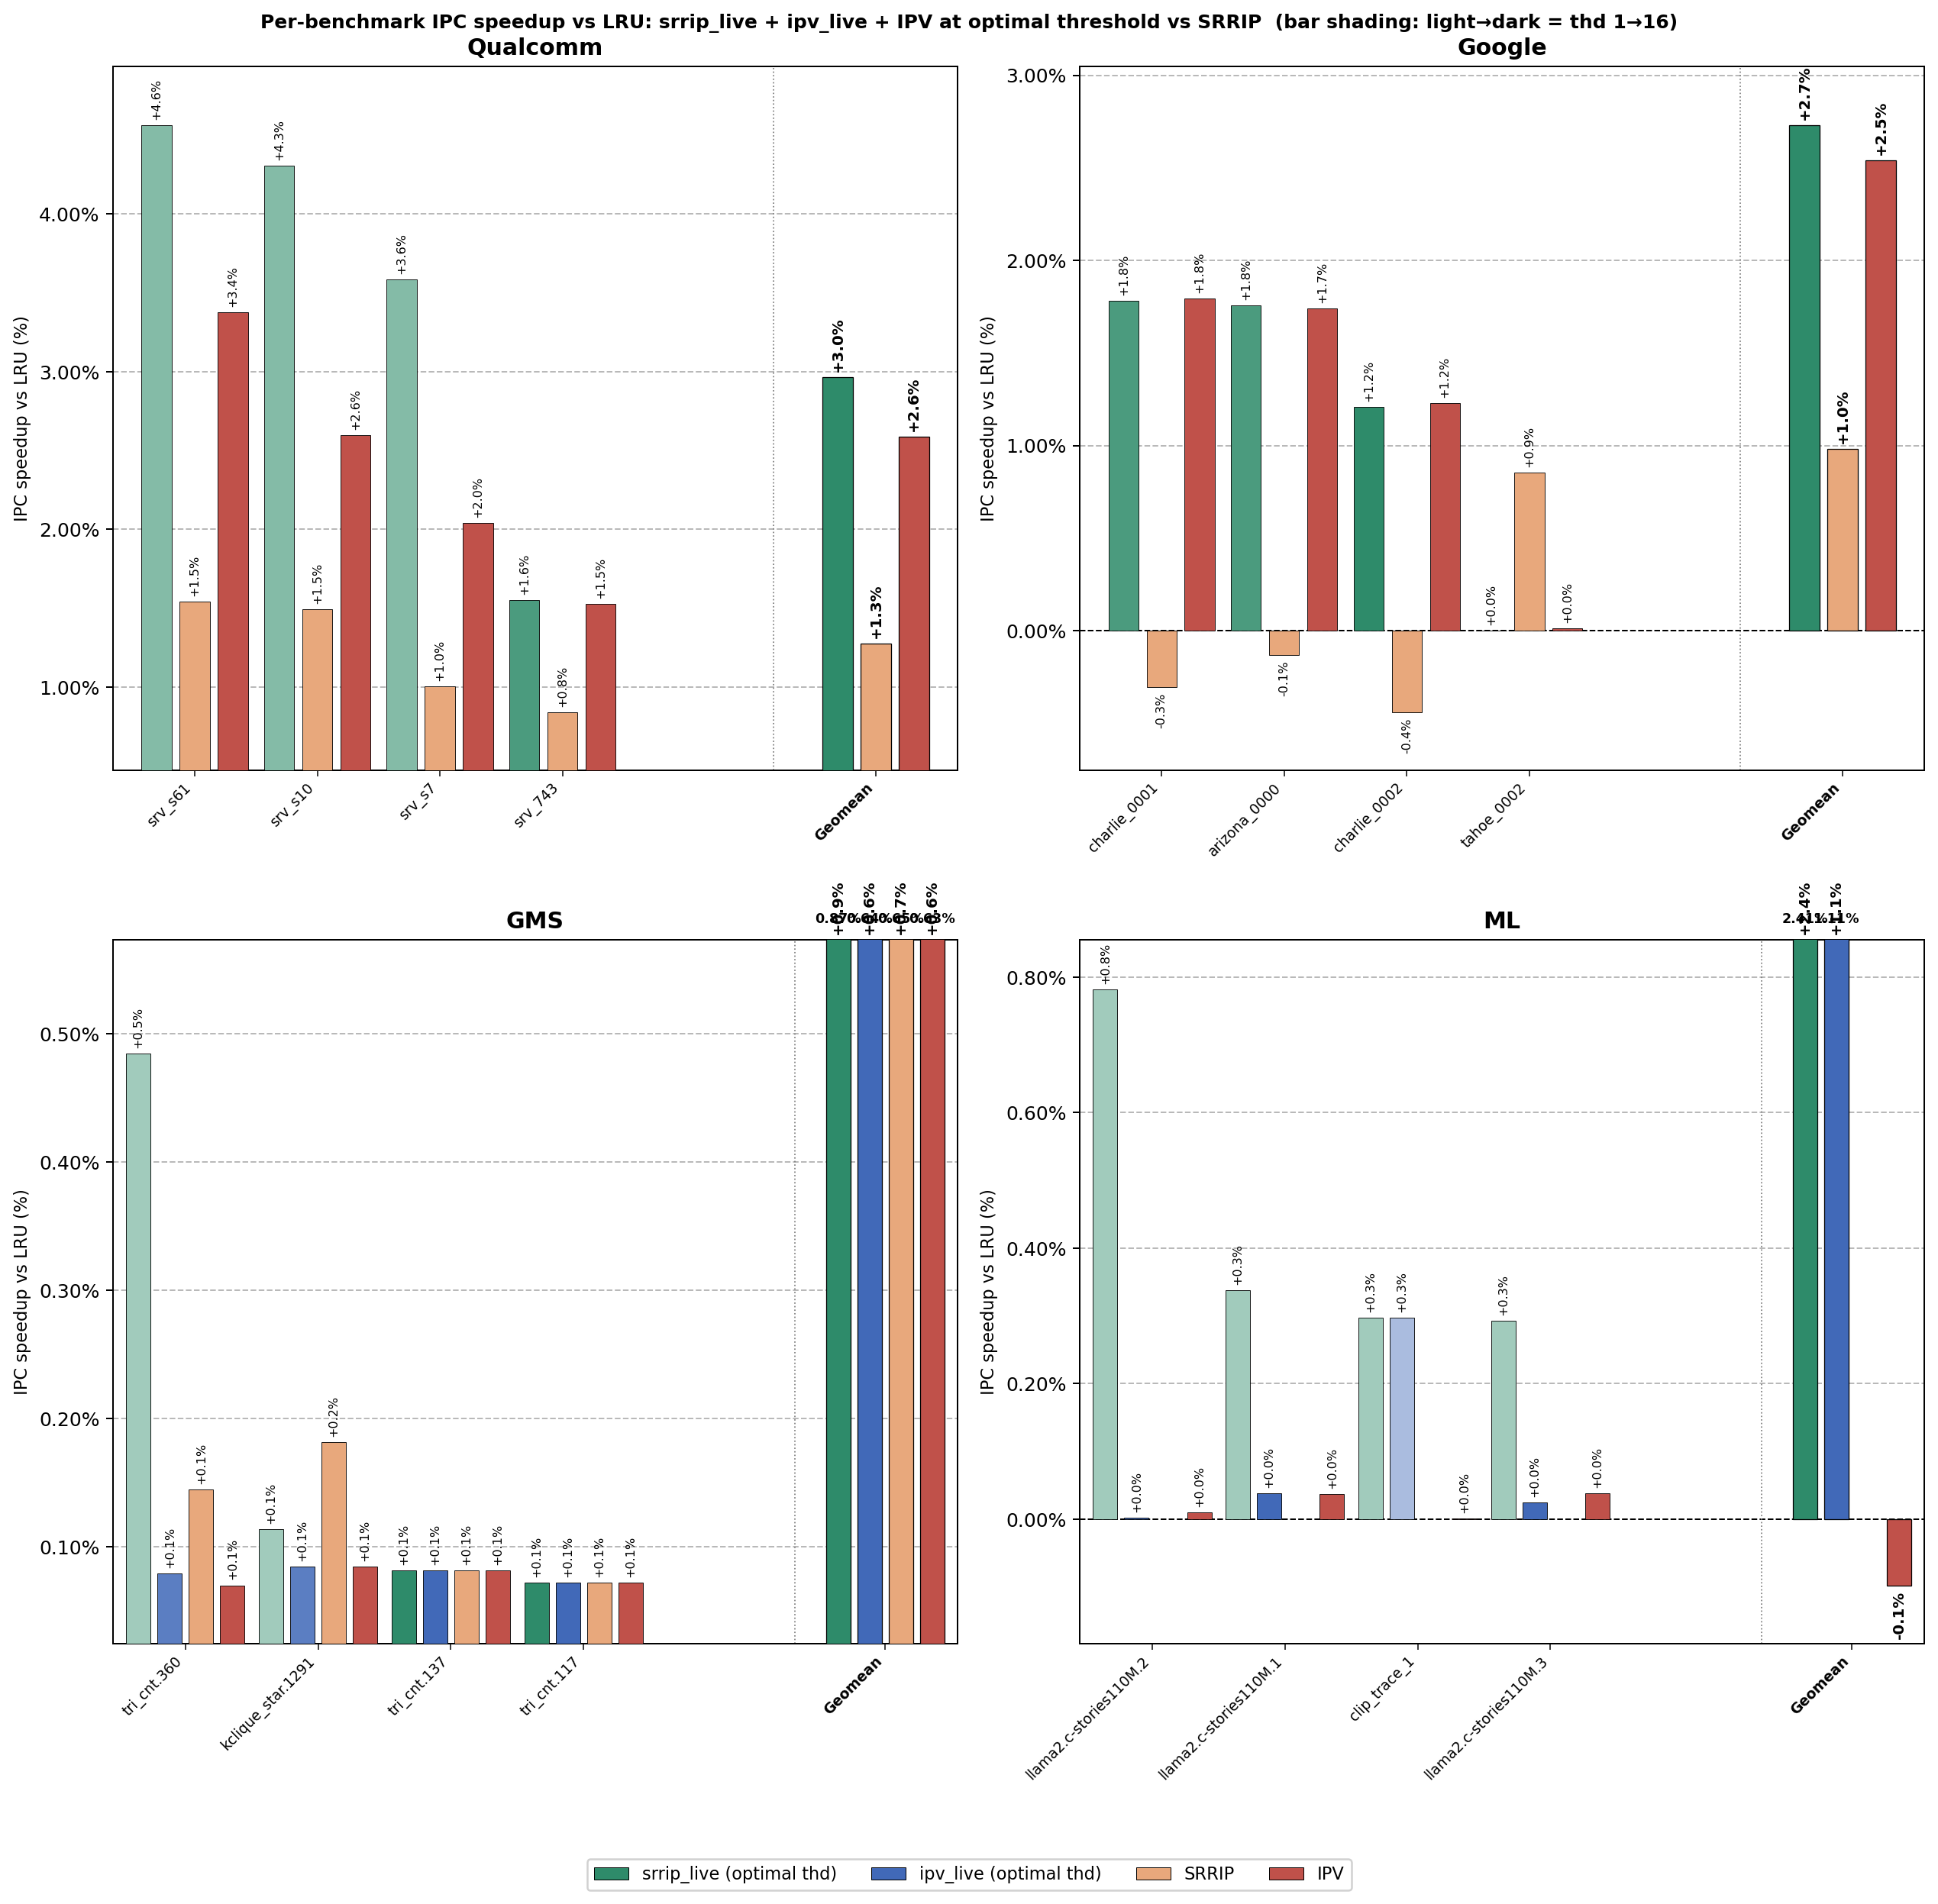
\includegraphics[width=\linewidth]{../../plots/optimal_thd_new_addr.png}
  \caption{As Figure~\ref{fig:srrip_live_thd_addr} for Qualcomm, Google,
           GMS, and AI/ML.  The AI/ML regression seen with PC-indexed
           history is eliminated: all AI/ML traces are near-neutral or
           positive.}
  \label{fig:srrip_live_thd_addr_new}
\end{figure}

\texttt{ipv\_live} replaces the scalar RRPV with a pair of learned vectors
--- one for insertion, one for promotion --- selected per fill based on the
liveness class of the filling PC.
Figure~\ref{fig:ipv_live} shows the suite-level comparison; per-workload
breakdowns are in Figures~\ref{fig:ipv_live_thd} and~\ref{fig:ipv_live_thd_new}.

\begin{figure}[htbp]
  \centering
  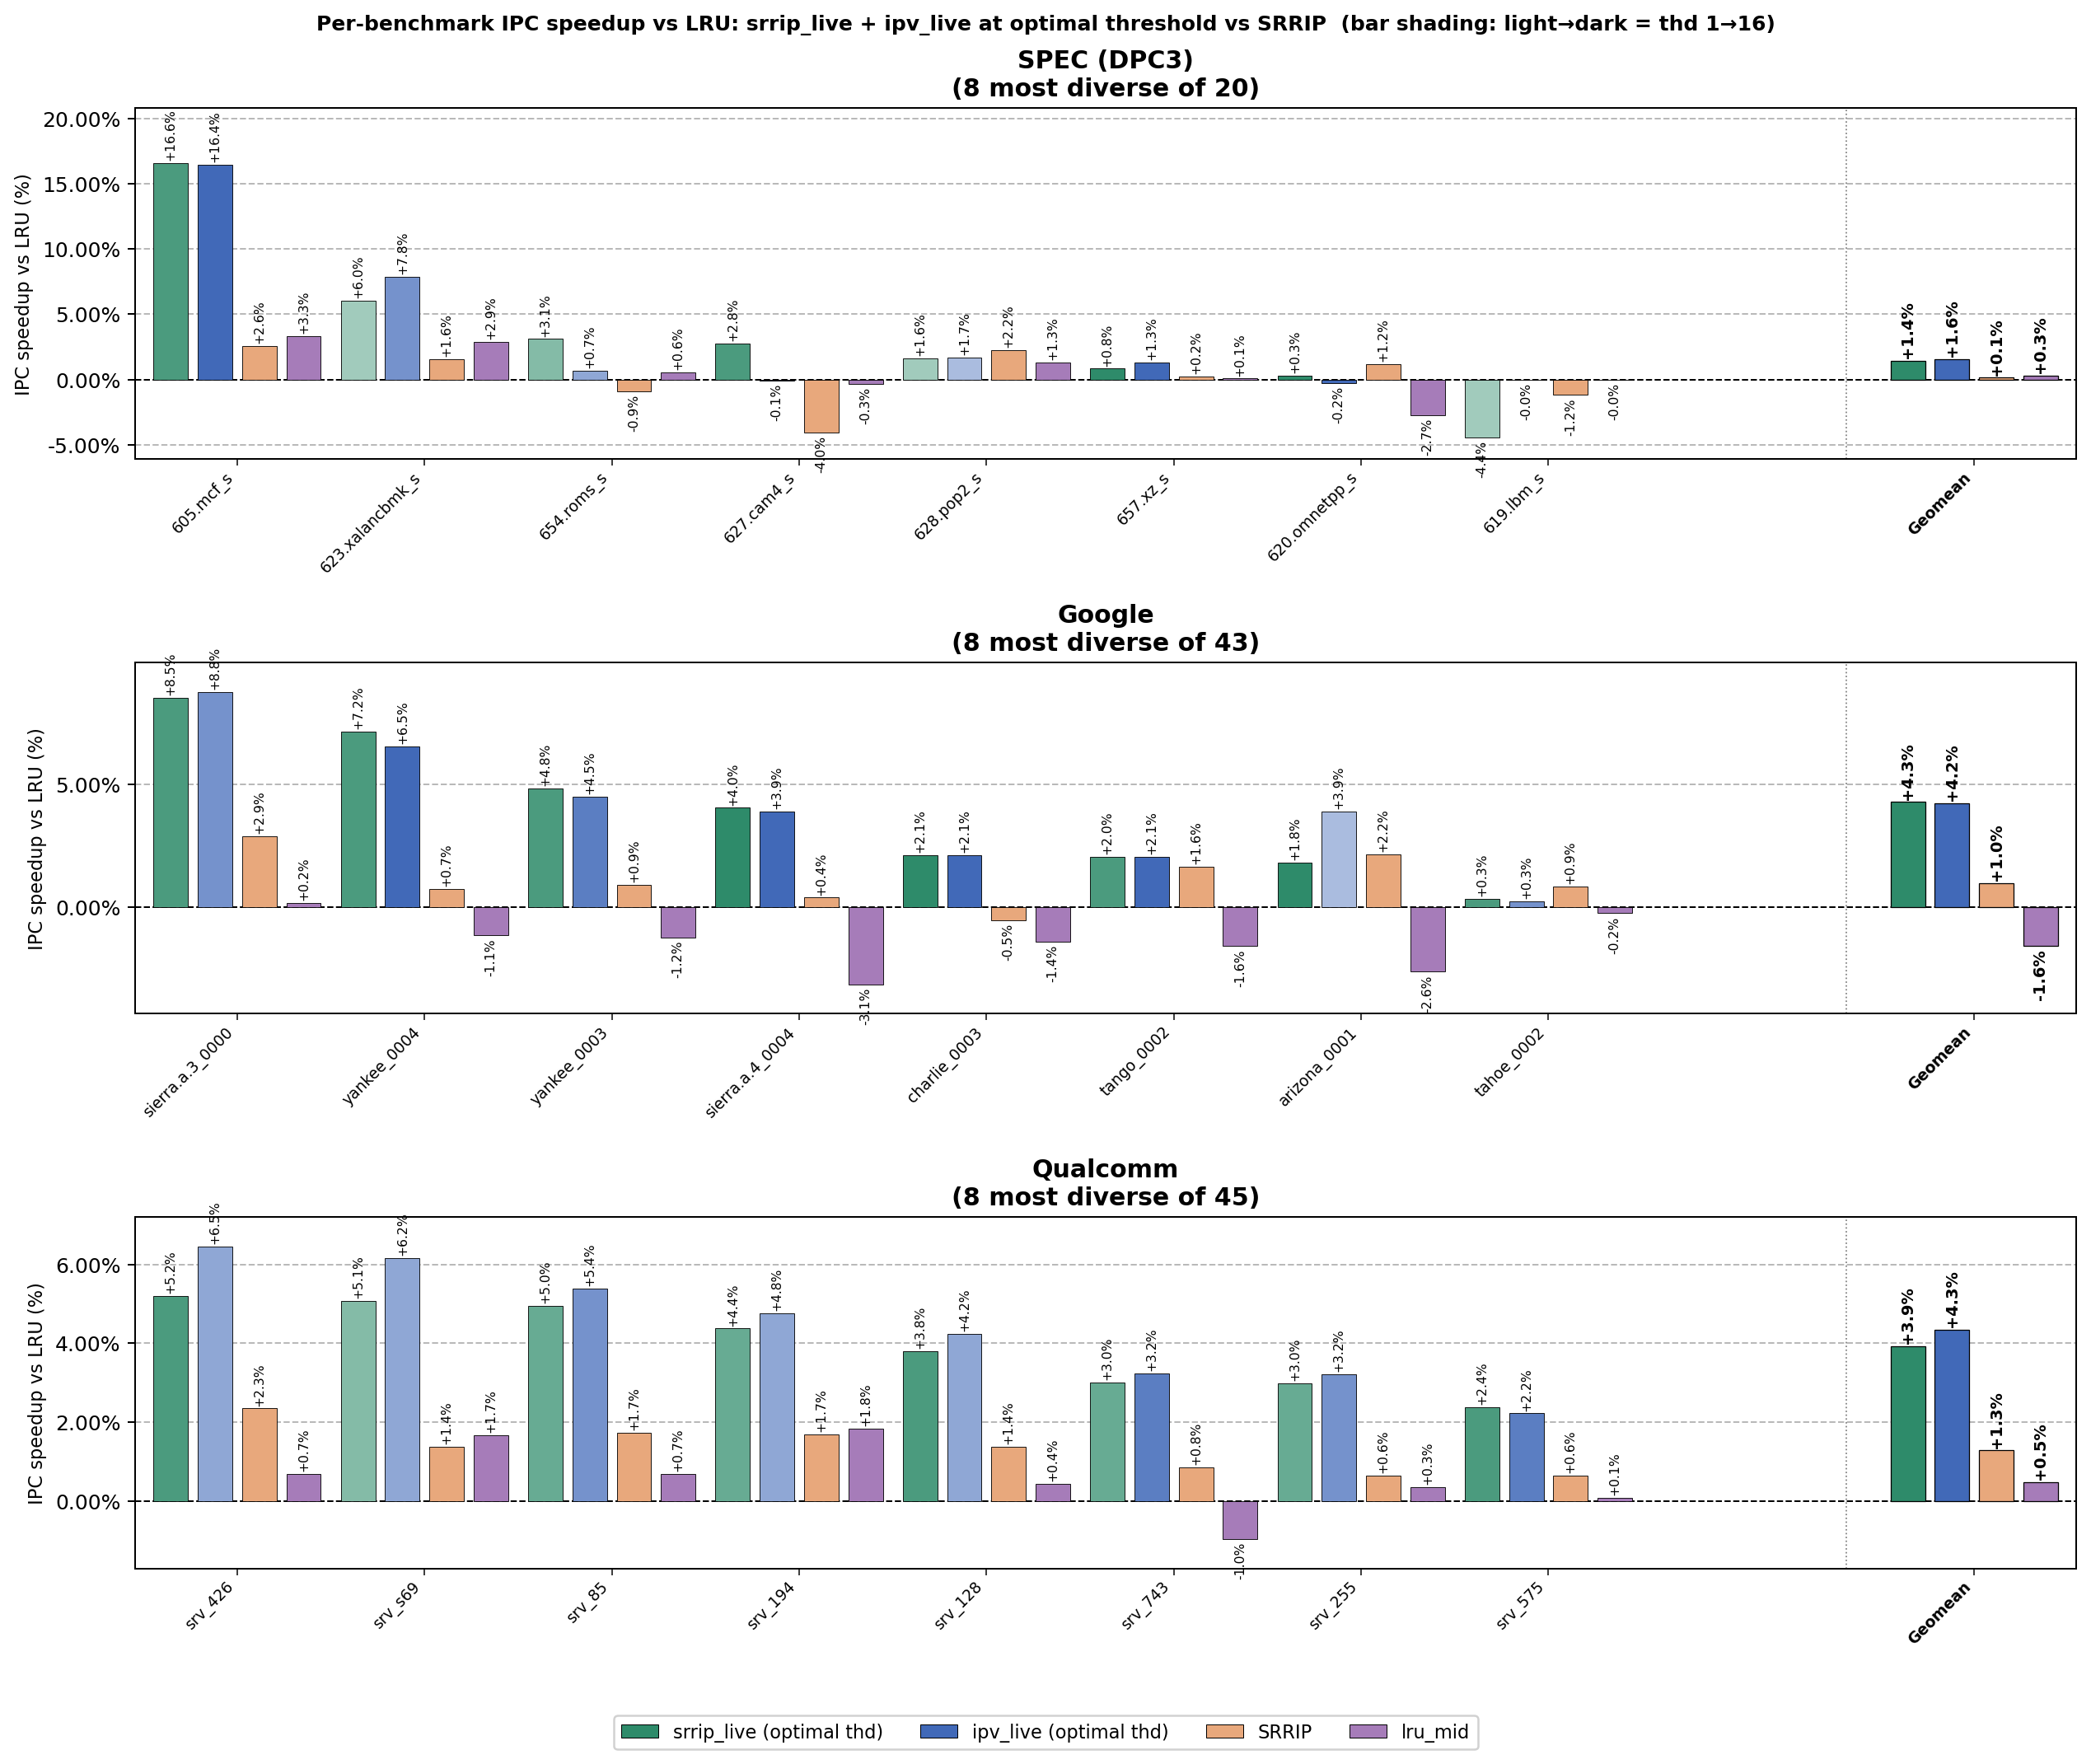
\includegraphics[width=\linewidth,height=0.38\textheight,keepaspectratio]{../../plots/ipv_live/ipv_live_all_suites.png}
  \caption{Geomean IPC speedup vs.\ LRU for SRRIP, IPV,
           \texttt{srrip\_live}, and \texttt{ipv\_live} across SPEC,
           Google, and Qualcomm, each at its per-suite optimal threshold.}
  \label{fig:ipv_live}
\end{figure}

\begin{figure}[htbp]
  \centering
  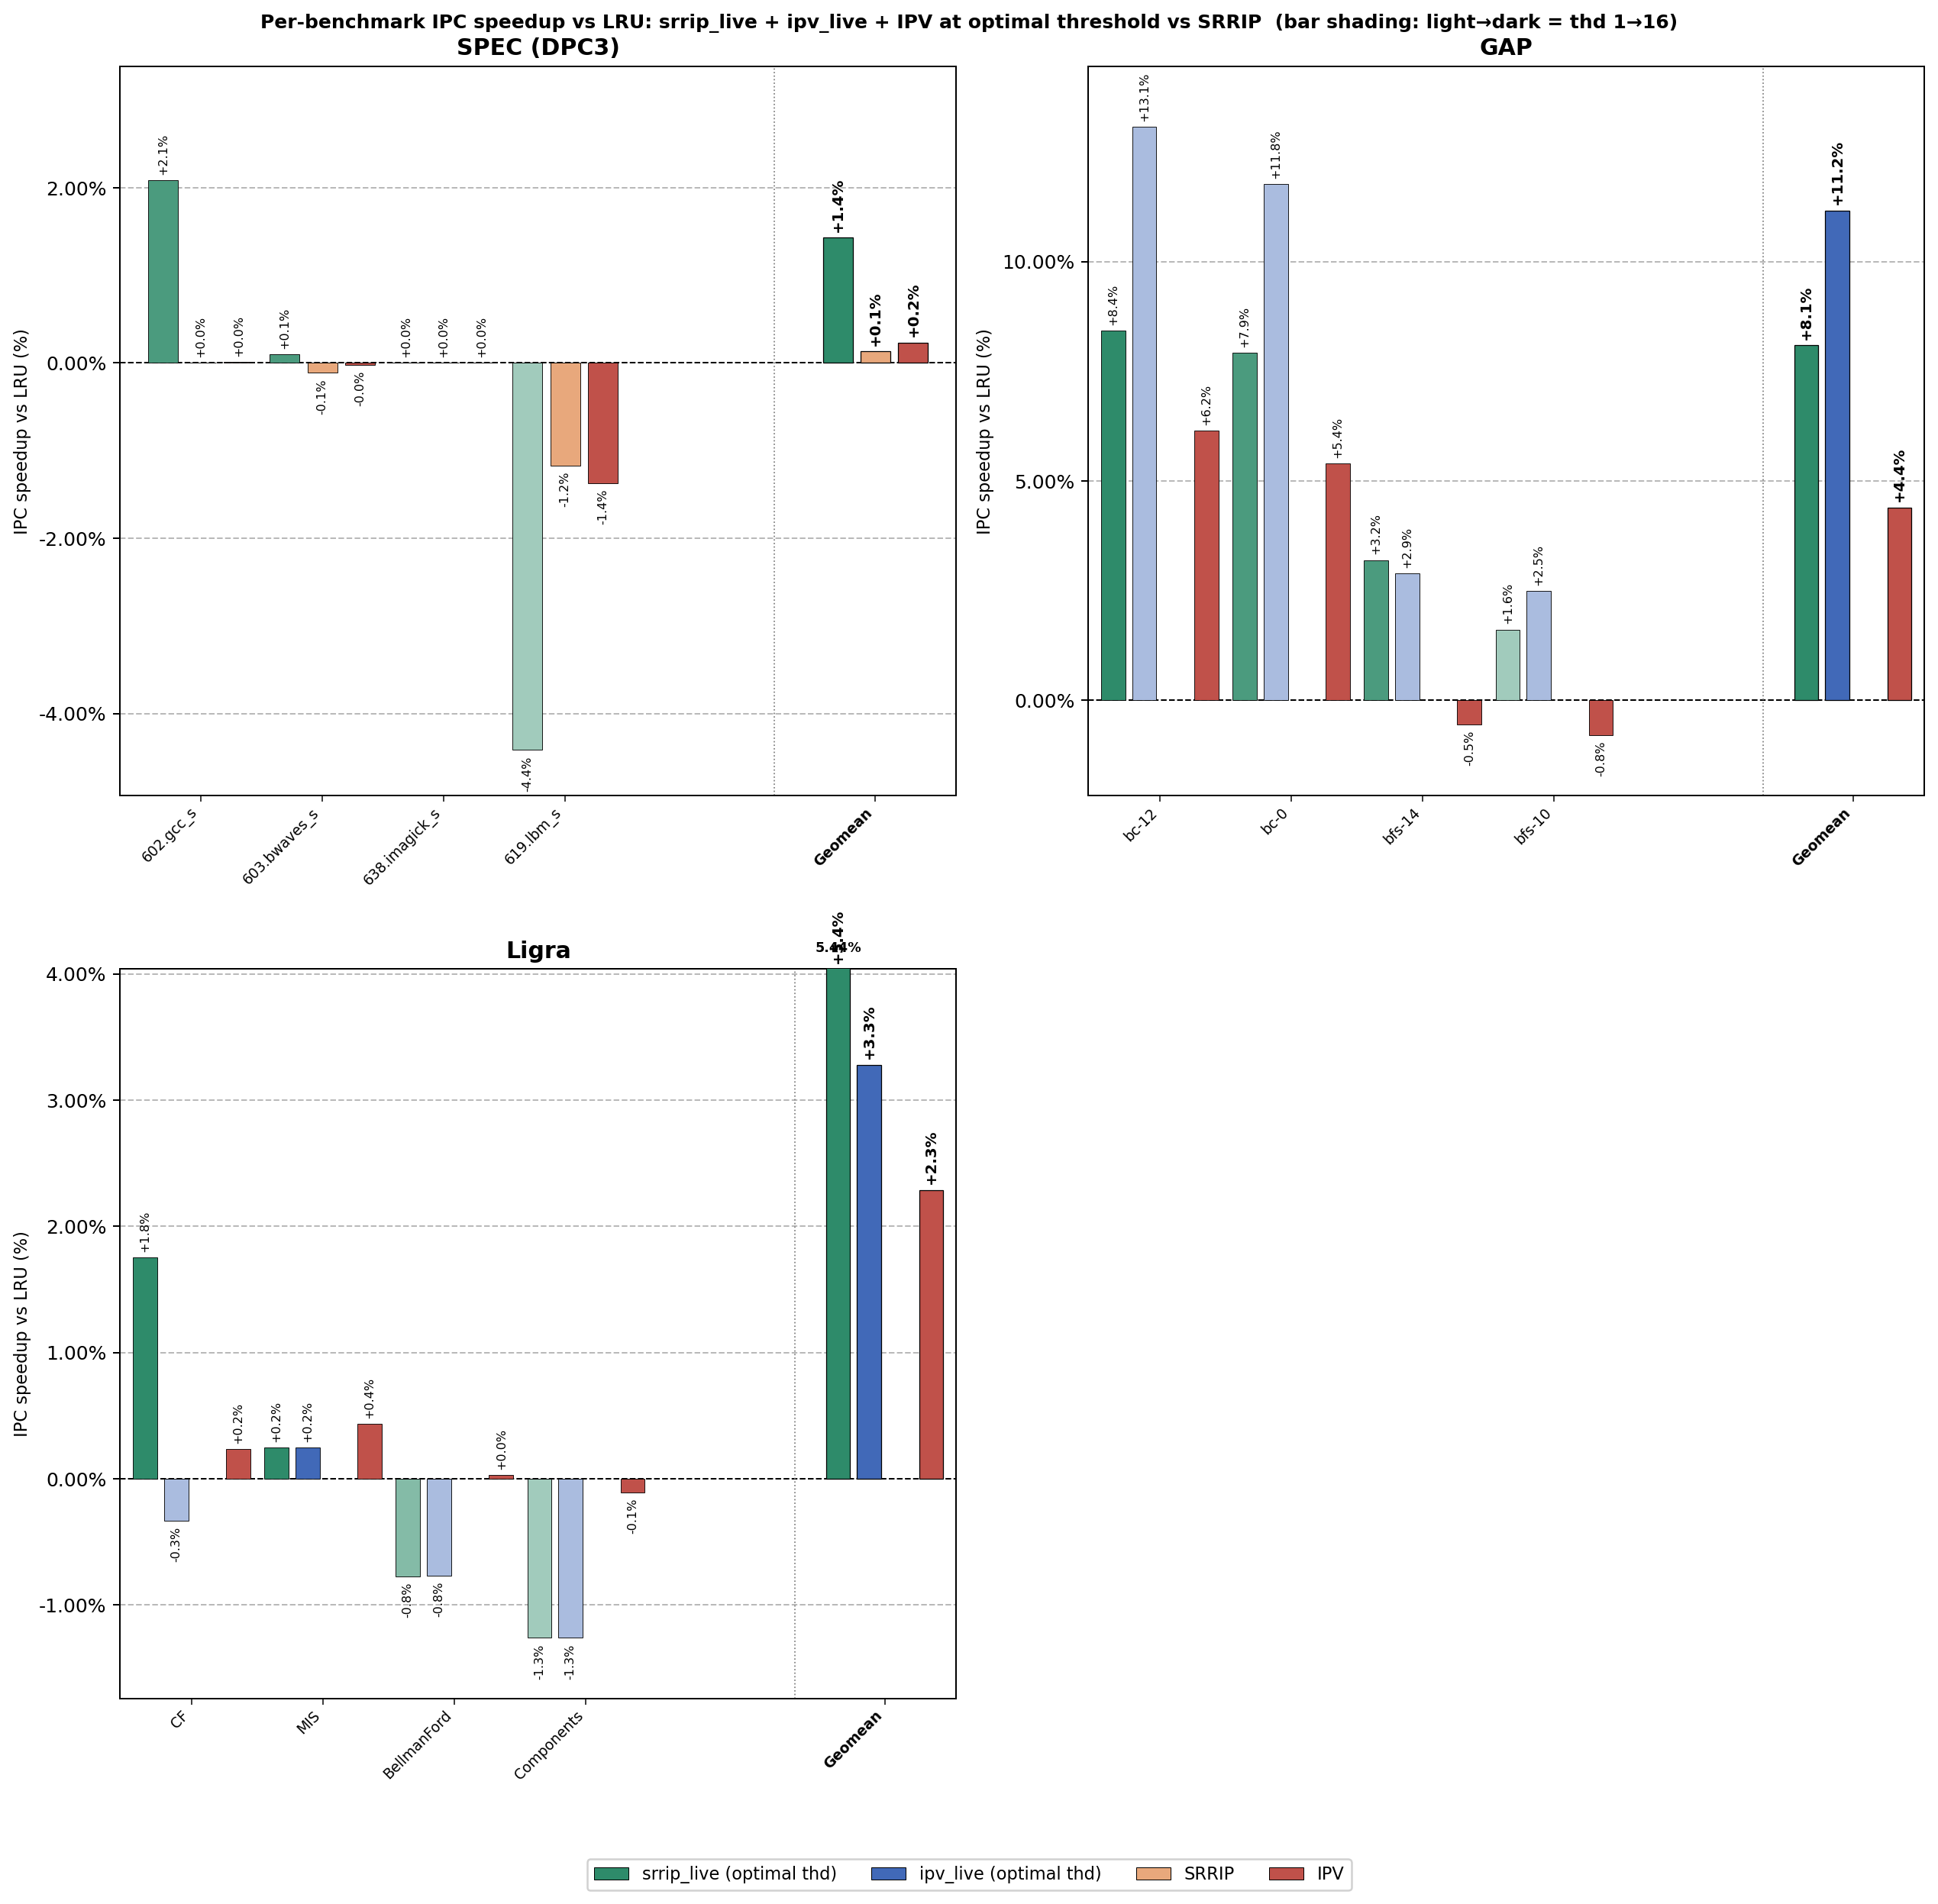
\includegraphics[width=\linewidth]{../../plots/optimal_thd_maz_srrip_ipv_pc.png}
  \caption{Per-workload IPC speedup vs.\ LRU for \texttt{srrip\_live}
           and \texttt{ipv\_live} (PC-indexed history) for SPEC, GAP,
           and Ligra.  \texttt{ipv\_live} bars shown where data is
           available (GAP, Ligra).
           Four workloads per suite plus suite geomean.}
  \label{fig:ipv_live_thd}
\end{figure}

\begin{figure}[htbp]
  \centering
  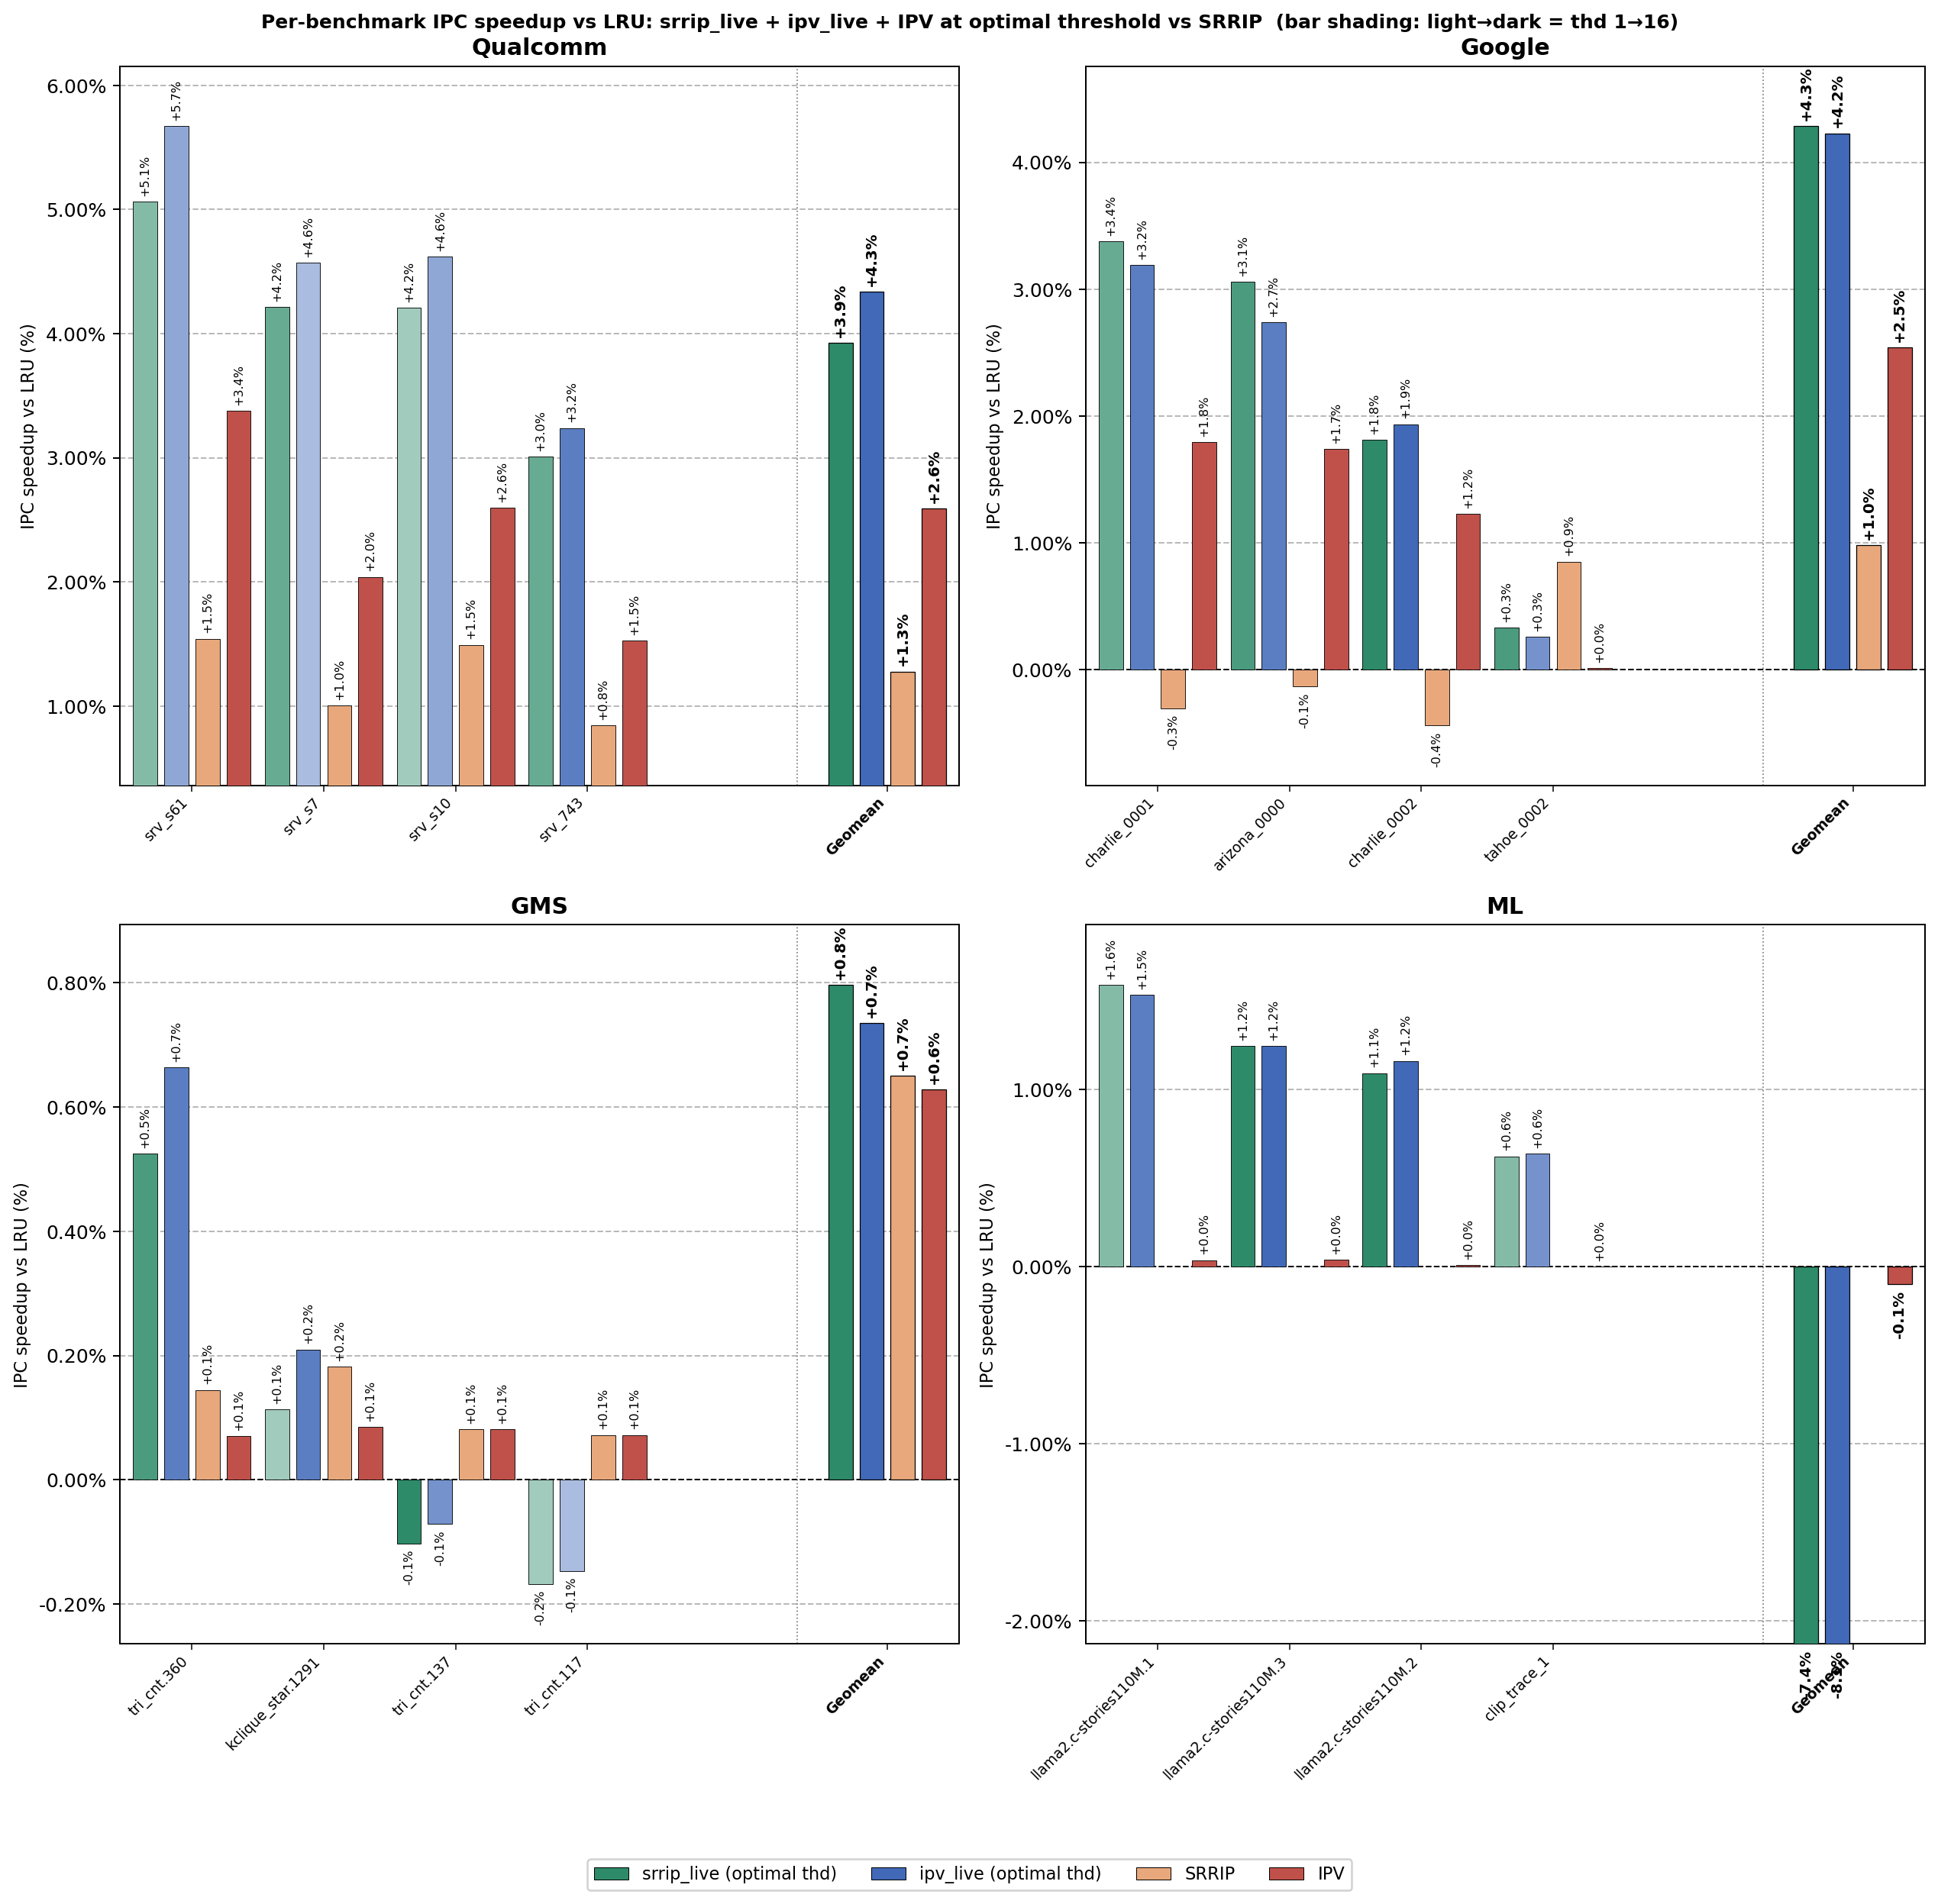
\includegraphics[width=\linewidth]{../../plots/optimal_thd_new_srrip_ipv_pc.png}
  \caption{As Figure~\ref{fig:ipv_live_thd} for Qualcomm, Google, GMS,
           and AI/ML.  \texttt{ipv\_live} bars shown where data is
           available (GMS, AI/ML).}
  \label{fig:ipv_live_thd_new}
\end{figure}

\texttt{ipv\_live} matches or exceeds \texttt{srrip\_live} on SPEC and
Qualcomm, but the margin is small.
Two differences stand out.

\textit{GAP benefits more with learned vectors.}
\texttt{ipv\_live} reaches $+11.2\%$ geomean at mid\_thd\,$= 1$ vs.\ $+7.9\%$
for \texttt{srrip\_live} at its optimal threshold, and it prefers
\emph{lower} thresholds.
GAP workloads have stable, concentrated access patterns where few
observations suffice to classify a PC's liveness, so the learned vectors
exploit the signal more aggressively than the scalar RRPV.

\textit{ipv\_live largely resolves the AI/ML regression.}
With PC-indexed history at mid\_thd\,$= 16$, the geomean speedup is $+2.2\%$
versus $-8.0\%$ for \texttt{srrip\_live} at the same setting.
The learned promotion vector appears more robust to non-stationary liveness
patterns: even when insertion-history is misleading, the policy can recover
partial benefit from the promotion signal.

\subsection{STLB-only: threshold sensitivity}
\label{sec:stlb_repl}

\todo{Add STLB-only threshold sweep figures (\texttt{stlb\_srrip\_live}
and \texttt{stlb\_ipv\_live}) for all seven suites.
Data from the stlb\_thd runs is available; plots pending.}

\subsection{Combined LLC+STLB replacement}
\label{sec:combined_repl}

The preceding experiments apply liveness-guided replacement to the LLC
alone.
A natural extension is to apply the same history-guided policy
simultaneously at the STLB, targeting dead TLB fills in the same way as
dead LLC fills.
The \texttt{srrip\_live\_both} and \texttt{ipv\_live\_both} configurations
do this: each level independently consults the shared \texttt{merged\_pc\_hist}
table and sets its RRPV or IPV vector accordingly.
The \texttt{stlb\_srrip\_live} and \texttt{stlb\_ipv\_live} variants apply
the policy at the STLB only (LLC reverts to LRU), and the \texttt{ipv} /
\texttt{ipv\_both} variants use the static IPV policy without per-PC
liveness history.

Figure~\ref{fig:combined_repl_all7} shows the geomean IPC speedup
vs.\ \texttt{srrip\_live\_both} for all seven suites.
The key observation is that applying liveness-guided replacement to both
levels is never worse than LLC-only, and provides small additional gains
on suites where the STLB dead-on-arrival correlation is high.
On suites where LLC and STLB DoA are weakly correlated (Google, Qualcomm,
GAP), the \texttt{\_both} variants match the LLC-only result closely,
as expected: the STLB history table provides no additional useful signal
beyond what the LLC already captures.

\begin{figure}[htbp]
  \centering
  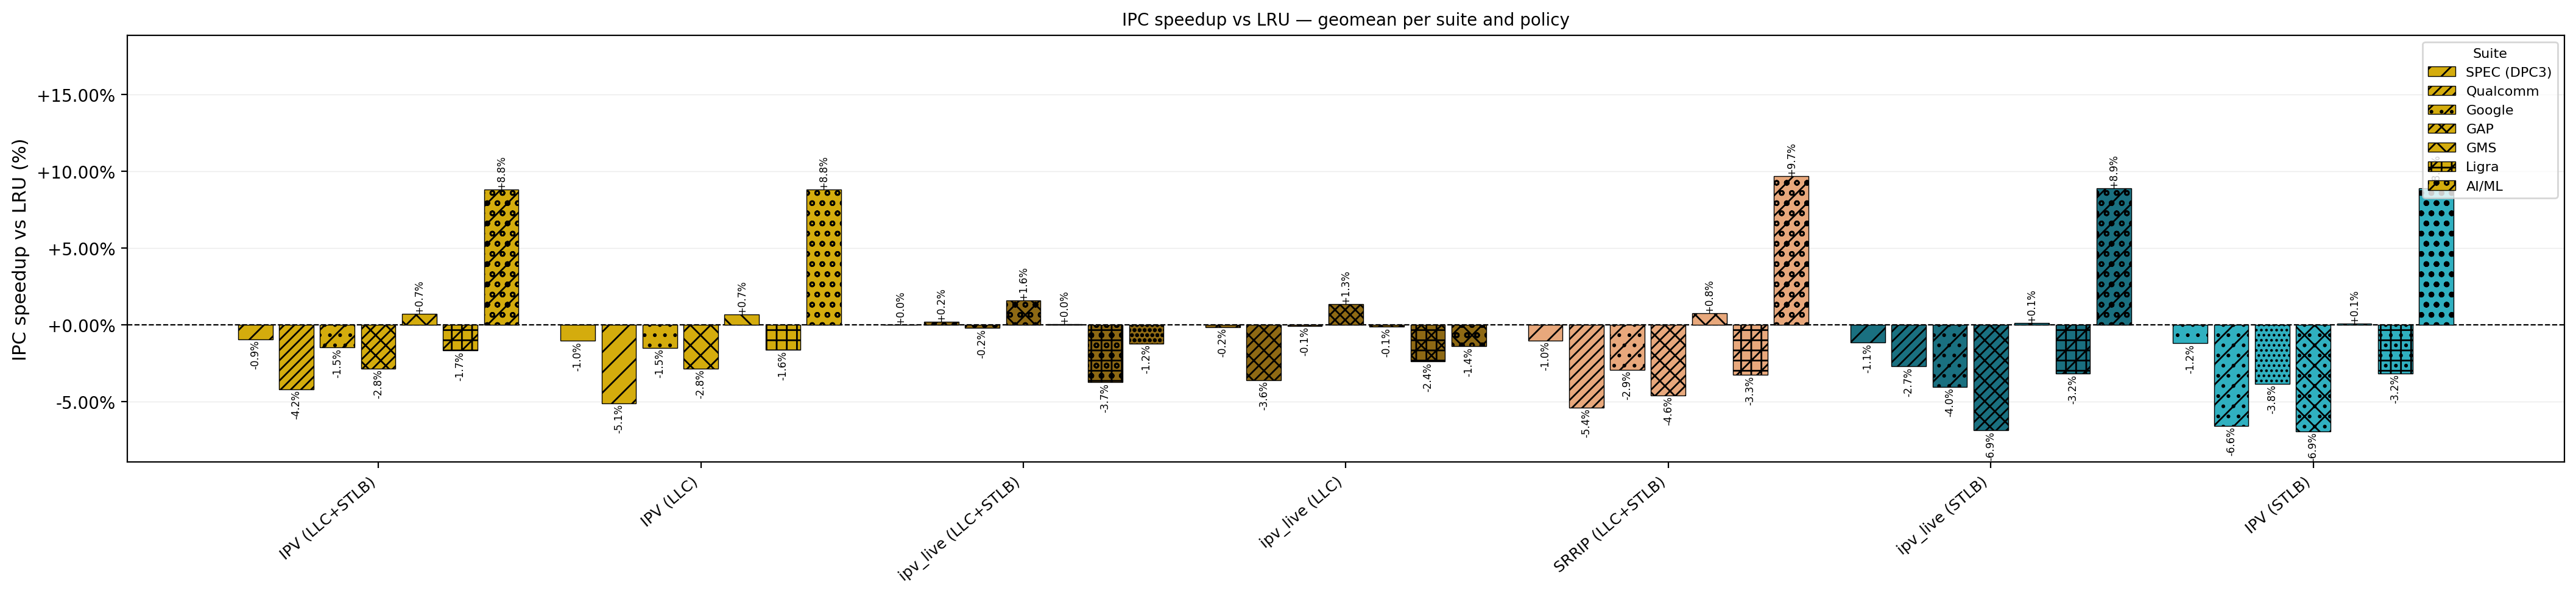
\includegraphics[width=\linewidth]{../../plots/combined_repl_all7.png}
  \caption{Combined LLC+STLB replacement policy comparison across all seven
           suites.  Geomean IPC speedup vs.\ \texttt{srrip\_live\_both}
           for LLC-only, STLB-only, and joint (LLC+STLB) variants of
           SRRIP, IPV, \texttt{srrip\_live}, and \texttt{ipv\_live}.}
  \label{fig:combined_repl_all7}
\end{figure}

% ─────────────────────────────────────────────────────────────────────────────
\section{Bypass Predictor: Mechanism and Variants}
\label{sec:bypass}
% ─────────────────────────────────────────────────────────────────────────────

\subsection{dpPred: STLB-level page bypass}

At each STLB page fault, dpPred decides whether the faulting page is
likely to be DoA.
It maintains a PC-indexed page-history table (\texttt{phist}) that counts
how often each faulting PC has produced pages whose STLB Accessed bit was
clear at check time (i.e.\ the page was never re-accessed after its fault
was handled).
When the counter for a given PC exceeds a confidence threshold
\texttt{pconf}, the faulting page frame number (PFN) is pushed into the
Page Frame Queue (PFQ, capacity~8).
The PFQ acts as a sliding window over the most recently predicted-DoA
pages; when full, the oldest entry is displaced.

\subsection{cbPred: LLC-level block bypass}

cbPred acts at LLC fill time.
It bypasses a fill if two conditions hold simultaneously: (1)~the block's
PFN is currently in the PFQ, meaning dpPred already predicted its page DoA,
and (2)~the block's own PC-indexed block-history counter (\texttt{bconf})
exceeds a threshold.
The double gate is conservative by design: requiring both a page-level and
a block-level prediction reduces false bypasses but also limits reach ---
a DoA LLC block whose page dpPred did not flag will never be bypassed.

\subsection{Variants and hashing comparison}
\label{sec:bypass_variants}

\todo{Compare PC-indexed history against address-hashed history for both
dpPred and cbPred.
Show that replacing the PC-indexed table with a simple address hash degrades
prediction quality, particularly for workloads with high inter-PC liveness
variance (SPEC), where the per-PC structure is essential.
Add per-suite speedup bars for hashing variants alongside the PC-indexed
baseline from Section~\ref{sec:bypass_perf}.}

\subsection{PFQ size study}
\label{sec:pfq_size}

\todo{Vary PFQ capacity across $\{4, 8, 16, 32, 64\}$ entries and measure
the resulting PFQ hit rate and IPC speedup per suite.
The central question is whether a larger PFQ can compensate for low
LLC--STLB DoA correlation (Google, Qualcomm, GAP).
The hypothesis is that it cannot: on low-correlation workloads the STLB
signal is fundamentally decoupled from LLC DoA, so more PFQ entries do not
increase the probability of a PFQ hit at fill time.
On high-correlation workloads (Ligra, AI/ML) the PFQ saturates quickly and
larger sizes provide diminishing returns.}

\subsection{bconf-only bypass and EMA-based adaptive gating}
\label{sec:bconf_only}

\begin{figure}[htbp]
  \centering
  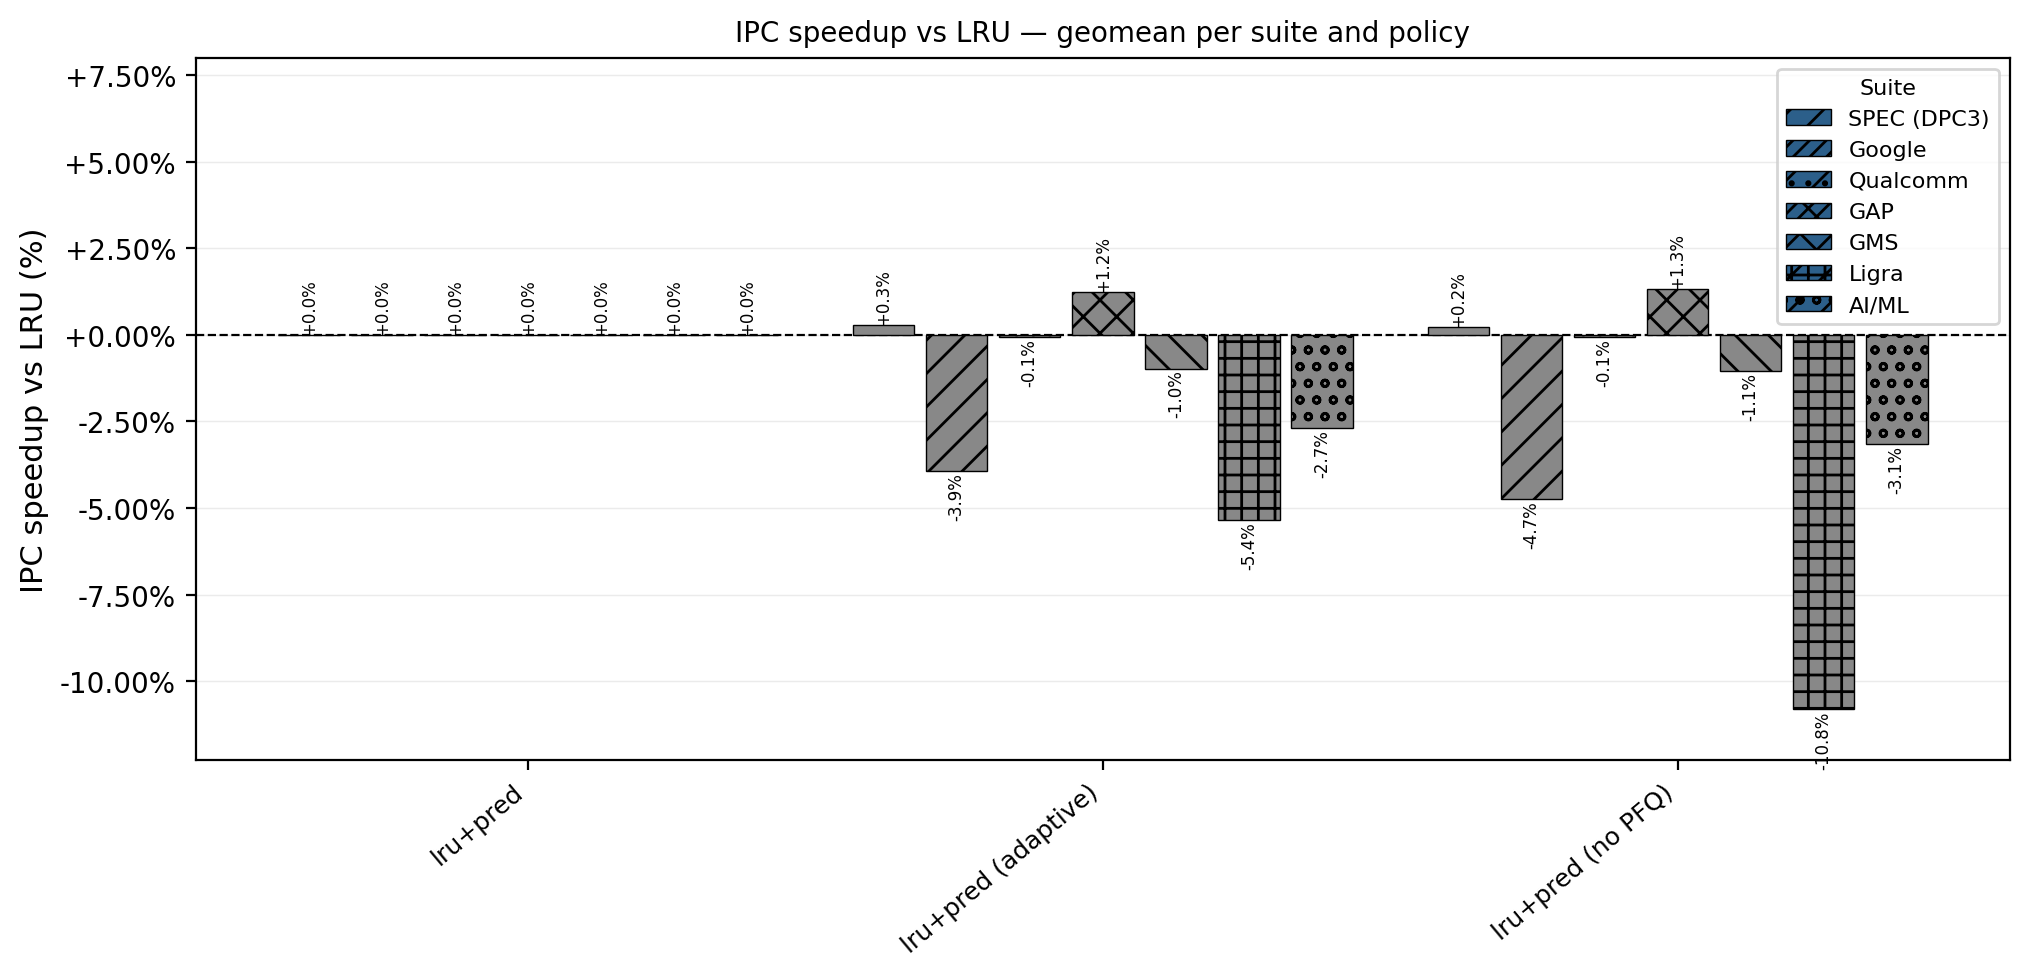
\includegraphics[width=\linewidth]{../../plots/pfq_gating/pfq_gating_all7_vs_pred.png}
  \caption{IPC speedup vs.\ the standard gated cbPred (\texttt{lru+pred}) for two
           relaxed gating strategies across all seven suites.
           \texttt{lru+pred (no PFQ)}: cbPred bypasses on block-level
           confidence alone, with no PFQ membership check.
           \texttt{lru+pred (adaptive)}: PFQ gate is enabled or disabled at
           runtime by an EMA of the PFQ hit rate
           (window\,=\,10\,000 fills, threshold\,=\,30\%).}
  \label{fig:pfq_gating}
\end{figure}

Figure~\ref{fig:pfq_gating} shows the effect of removing or adaptively
relaxing the PFQ membership requirement.
The two strategies have opposite effects on high- and low-correlation
workloads, and neither dominates the standard gated cbPred across all
seven suites.

\emph{bconf-only (no PFQ gate).}
Removing the PFQ requirement frees cbPred to bypass on block-level
confidence alone.
On GAP (${\sim}1\%$ correlation) this yields a small gain
($+1.3\%$): the PFQ was rarely populated with the right PFN, so the gate
was blocking bypasses that the block-level history correctly identified as
DoA.
SPEC and Qualcomm are negligibly affected ($+0.2\%$ and $-0.1\%$).
On high-correlation workloads, however, removing the gate is harmful:
Ligra regresses by $-10.8\%$, Google by $-4.7\%$, and AI/ML by $-3.1\%$.
The interpretation is that the PFQ gate provides essential precision on
those suites --- it acts as a filter that ensures cbPred only bypasses
blocks whose page was already flagged DoA by dpPred.
Without it, block-level \texttt{bconf} alone is too aggressive, bypassing
blocks that would otherwise be hits, particularly on streaming workloads
where a small number of live PCs intermix with predominantly dead ones.

\emph{EMA-based adaptive gating.}
The adaptive variant monitors the PFQ hit rate via an exponential moving
average over the most recent 10\,000 LLC fills.
When the hit rate falls below 30\%, the PFQ gate is disabled; when it
rises above, PFQ membership is required.
The EMA consistently reduces the regression vs.\ bconf-only: Ligra
improves from $-10.8\%$ to $-5.4\%$, and AI/ML from $-3.1\%$ to
$-2.7\%$.
This confirms that the EMA correctly detects the high PFQ hit rate on
high-correlation workloads and re-enables the gate.
GAP's gain shrinks slightly ($+1.2\%$ vs.\ $+1.3\%$ for no-PFQ) because
the EMA also occasionally re-enables the gate during phases when the PFQ
hit rate is transiently elevated.

Neither strategy matches the standard gated cbPred across all suites.
The remaining regression on Ligra ($-5.4\%$) and AI/ML ($-2.7\%$)
suggests that the EMA window and threshold parameters used here are not
optimally tuned, or that a fundamentally different correlation proxy is
needed at fill time.
The standard gated cbPred, with its static PFQ window, outperforms both
alternatives on the suites where it matters most (high-correlation), while
the no-PFQ and adaptive variants offer only marginal improvement on
low-correlation suites (GAP $+1.2$--$1.3\%$) at the cost of regressions
elsewhere.
The PFQ gate appears to be a net positive mechanism in the current design.

% ─────────────────────────────────────────────────────────────────────────────
\section{Synthesis}
\label{sec:synthesis}
% ─────────────────────────────────────────────────────────────────────────────

Table~\ref{tab:mechanism_fit} summarises the observed and anticipated
effectiveness of each mechanism by workload class.
LLC replacement policy results and LLC--STLB DoA correlation measurements
are now complete for all seven suites.
Bypass predictor results remain pending for GAP, Ligra, and AI/ML;
GMS bypass predictor data is available and shows near-neutral gain
consistent with its $\approx9\%$ correlation.

\begin{table}[htbp]
  \centering
  \caption{Mechanism effectiveness by workload class.
           $+$ helpful; $\circ$ neutral; $-$ harmful;
           \textbf{!} sensitive to indexing/threshold.
           \textbf{?} awaiting data.
           $^\dagger$ Graph DoA correlation varies widely:
           GAP $\approx1\%$, GMS $\approx9\%$, Ligra $\approx100\%$.}
  \label{tab:mechanism_fit}
  \begin{tabular}{lcccc}
    \toprule
                                    & SPEC        & Server      & Graph       & AI/ML       \\
    \midrule
    DoA correlation (STLB$\to$LLC)  & high        & near zero   & mixed$^\dagger$ & very high   \\
    \midrule
    dpPred (STLB bypass)            & $+$         & $\circ$     & \textbf{?}  & \textbf{?}  \\
    cbPred (LLC bypass, PFQ-gated)  & $+$         & $\circ$     & \textbf{?}  & \textbf{?}  \\
    \texttt{srrip\_live} (PC-idx)   & $+$         & $+$         & $++$        & $-$\textbf{!} \\
    \texttt{srrip\_live} (addr-idx) & $+$         & $+$         & $+$         & $\circ$\textbf{!} \\
    \texttt{ipv\_live} (PC-idx)     & $+$         & $+$         & $++$        & $+$\textbf{!} \\
    \bottomrule
  \end{tabular}
\end{table}

The LLC--STLB DoA correlation is the central explanatory variable: it
predicts bypass predictor effectiveness precisely, separating workloads
where the page-level signal is useful (SPEC, Ligra, AI/ML) from those
where it is not (server suites, GAP).
Block-level replacement policy (\texttt{srrip\_live}) recovers the signal
lost at the page level, benefiting all workload classes including
low-correlation ones.
The key open question is whether relaxing the cbPred gate
(Section~\ref{sec:bconf_only}) yields gains on low-correlation workloads
comparable to those already achieved by \texttt{srrip\_live}.

\end{document}
